\documentclass{beamer}
\mode<presentation>{
  \usetheme{Boadilla}
  \usefonttheme[onlylarge]{structurebold}
  \usefonttheme[stillsansseriflarge]{serif}
  \setbeamerfont*{frametitle}{size=\normalsize,series=\bfseries}
  % \setbeamertemplate{navigation symbols}{}
  \setbeamercovered{transparent}
}
\usepackage[english]{babel}
\usepackage[latin1]{inputenc}
\usepackage{times}
\usepackage[T1]{fontenc}
\usepackage{amsmath}
\usepackage{amssymb}
\usepackage{esint}
\usepackage{hyperref}
\usepackage{tikz}
\usepackage{xkeyval}
\usepackage{xargs}
\usepackage{xcolor}
\usepackage{verbatim}
\usepackage{listings}
\usepackage{multimedia}
\usepackage{bm}
\usepackage{siunitx}
\usetikzlibrary{
  arrows,
  calc,
  decorations.pathmorphing,
  decorations.pathreplacing,
  decorations.markings,
  fadings,
  positioning,
  shapes,
  arrows.meta
}
\usepgfmodule{oo}

\pgfdeclareradialshading{glow2}{\pgfpoint{0cm}{0cm}}{
  color(0mm)=(white);
  color(2mm)=(white);
  color(8mm)=(black);
  color(10mm)=(black)
}
\pgfdeclareradialshading{glow}{\pgfpoint{0cm}{0cm}}{
  color(0mm)=(white);
  color(5mm)=(white);
  color(9mm)=(black);
  color(10mm)=(black)
}

\begin{tikzfadingfrompicture}[name=glow fading]
  \shade [shading=glow] (0,0) circle (1);
\end{tikzfadingfrompicture}

\begin{tikzfadingfrompicture}[name=glow2 fading]
  \shade [shading=glow2] (0,0) circle (1);
\end{tikzfadingfrompicture}

\mode<handout>{
  \usepackage{pgfpages}
  \pgfpagesuselayout{4 on 1}[a4paper,landscape,border shrink=5mm]
  \setbeamercolor{background canvas}{bg=black!10}
}

\newcommand\pgfmathsinandcos[3]{%
  \pgfmathsetmacro#1{sin(#3)}%
  \pgfmathsetmacro#2{cos(#3)}%
}
\newcommand\LongitudePlane[3][current plane]{%
  \pgfmathsinandcos\sinEl\cosEl{#2} % elevation
  \pgfmathsinandcos\sint\cost{#3} % azimuth
  \tikzset{#1/.estyle={cm={\cost,\sint*\sinEl,0,\cosEl,(0,0)}}}
}
\newcommand\LatitudePlane[3][current plane]{%
  \pgfmathsinandcos\sinEl\cosEl{#2} % elevation
  \pgfmathsinandcos\sint\cost{#3} % latitude
  \pgfmathsetmacro\yshift{\cosEl*\sint}
  \tikzset{#1/.estyle={cm={\cost,0,0,\cost*\sinEl,(0,\yshift)}}} %
}
\newcommand\DrawLongitudeCircle[2][1]{
  \LongitudePlane{\angEl}{#2}
  \tikzset{current plane/.prefix style={scale=#1}}
  % angle of "visibility"
  \pgfmathsetmacro\angVis{atan(sin(#2)*cos(\angEl)/sin(\angEl))} %
  \draw[current plane] (\angVis:1) arc (\angVis:\angVis+180:1);
  \draw[current plane,dashed] (\angVis-180:1) arc (\angVis-180:\angVis:1);
}
\newcommand\DrawLatitudeCircleArrow[2][1]{
  \LatitudePlane{\angEl}{#2}
  \tikzset{current plane/.prefix style={scale=#1}}
  \pgfmathsetmacro\sinVis{sin(#2)/cos(#2)*sin(\angEl)/cos(\angEl)}
  % angle of "visibility"
  \pgfmathsetmacro\angVis{asin(min(1,max(\sinVis,-1)))}
  \draw[current plane,decoration={markings, mark=at position 0.6 with {\arrow{<}}},postaction={decorate},line width=.6mm] (\angVis:1) arc (\angVis:-\angVis-180:1);
  \draw[current plane,dashed,line width=.6mm] (180-\angVis:1) arc (180-\angVis:\angVis:1);
}
\newcommand\DrawLatitudeCircle[2][1]{
  \LatitudePlane{\angEl}{#2}
  \tikzset{current plane/.prefix style={scale=#1}}
  \pgfmathsetmacro\sinVis{sin(#2)/cos(#2)*sin(\angEl)/cos(\angEl)}
  % angle of "visibility"
  \pgfmathsetmacro\angVis{asin(min(1,max(\sinVis,-1)))}
  \draw[current plane] (\angVis:1) arc (\angVis:-\angVis-180:1);
  \draw[current plane,dashed] (180-\angVis:1) arc (180-\angVis:\angVis:1);
}
\newcommand\coil[1]{
  {\rh * cos(\t * pi r)}, {\apart * (2 * #1 + \t) + \rv * sin(\t * pi r)}
}
\makeatletter
\define@key{DrawFromCenter}{style}[{->}]{
  \tikzset{DrawFromCenterPlane/.style={#1}}
}
\define@key{DrawFromCenter}{r}[1]{
  \def\@R{#1}
}
\define@key{DrawFromCenter}{center}[(0, 0)]{
  \def\@Center{#1}
}
\define@key{DrawFromCenter}{theta}[0]{
  \def\@Theta{#1}
}
\define@key{DrawFromCenter}{phi}[0]{
  \def\@Phi{#1}
}
\presetkeys{DrawFromCenter}{style, r, center, theta, phi}{}
\newcommand*\DrawFromCenter[1][]{
  \setkeys{DrawFromCenter}{#1}{
    \pgfmathsinandcos\sint\cost{\@Theta}
    \pgfmathsinandcos\sinp\cosp{\@Phi}
    \pgfmathsinandcos\sinA\cosA{\angEl}
    \pgfmathsetmacro\DX{\@R*\cost*\cosp}
    \pgfmathsetmacro\DY{\@R*(\cost*\sinp*\sinA+\sint*\cosA)}
    \draw[DrawFromCenterPlane] \@Center -- ++(\DX, \DY);
  }
}
\newcommand*\DrawFromCenterText[2][]{
  \setkeys{DrawFromCenter}{#1}{
    \pgfmathsinandcos\sint\cost{\@Theta}
    \pgfmathsinandcos\sinp\cosp{\@Phi}
    \pgfmathsinandcos\sinA\cosA{\angEl}
    \pgfmathsetmacro\DX{\@R*\cost*\cosp}
    \pgfmathsetmacro\DY{\@R*(\cost*\sinp*\sinA+\sint*\cosA)}
    \draw[DrawFromCenterPlane] \@Center -- ++(\DX, \DY) node {#2};
  }
}
\makeatother

% not mandatory, but I though it was better to set it blank
\setbeamertemplate{headline}{}
\def\beamer@entrycode{\vspace{-\headheight}}

\tikzstyle{snakearrow} = [decorate, decoration={pre length=0.2cm,
  post length=0.2cm, snake, amplitude=.4mm,
  segment length=2mm},thick, ->]

%% document-wide tikz options and styles

\tikzset{%
  % >=latex, % option for nice arrows
  inner sep=0pt,%
  outer sep=2pt,%
  mark coordinate/.style={inner sep=0pt,outer sep=0pt,minimum size=3pt,
    fill=black,circle}%
}
\tikzset{
  % Define standard arrow tip
  >=stealth',
  % Define style for boxes
  punkt/.style={
    rectangle,
    rounded corners,
    draw=black, very thick,
    text width=8em,
    minimum height=2.5em,
    text centered},
}

\tikzset{onslide/.code args={<#1>#2}{%
    \only<#1>{\pgfkeysalso{#2}}
    % \pgfkeysalso doesn't change the path
  }}
\tikzset{alt/.code args={<#1>#2#3}{%
    \alt<#1>{\pgfkeysalso{#2}}{\pgfkeysalso{#3}}
    % \pgfkeysalso doesn't change the path
  }}
\tikzset{temporal/.code args={<#1>#2#3#4}{%
    \temporal<#1>{\pgfkeysalso{#2}}{\pgfkeysalso{#3}}{\pgfkeysalso{#4}}
    % \pgfkeysalso doesn't change the path
  }}

\makeatletter
\newbox\@backgroundblock
\newenvironment{backgroundblock}[2]{%
  \global\setbox\@backgroundblock=\vbox\bgroup%
  \unvbox\@backgroundblock%
  \vbox to0pt\bgroup\vskip#2\hbox to0pt\bgroup\hskip#1\relax%
}{\egroup\egroup\egroup}
\addtobeamertemplate{background}{\box\@backgroundblock}{}
\makeatother

\ifpdf
% Ensure reproducible output
\pdfinfoomitdate=1
\pdfsuppressptexinfo=-1
\pdftrailerid{}
\fi

\title{Building Single Molecules from Single Atoms}
\date{Jul. 2020}
\author{Yichao Yu}
\institute{Ni Group/Harvard}

%%% Outline

%% Goal
% New system and tool for quantum computing and quantum simulation
% Requires quantum system that is
% * Fully controllable
% * Allow entanglement
% * Scalable (to tens or hundreds)

%% System
% Many other systems in AMO
% Each approaches all have their advantages and disadvantages.
% These are the properties that we exploid and the reasons that we pick our system.
% Just like other systems they have their difficulties and that'll be the main focus of my talk.

% Molecules
% * Dipole intraction
% %% Strong, tunable, helps with achieving fast interaction
% %% while maintaining long coherence time.
% * Rich internal states (e.g. qubit state selection)

% Tweezers
% * Single site detection
% * Single site manipulation

% Two approaches (Cooling molecules vs forming molecules)
% (given our goal of combining optical tweezer with ultracold molecules)
% * Cooling molecules (show CaF picture)
% %% Difficulty on achieving lower temperature
% * Assembly (....)
% %% Difficulty on forming the molecule
% %% Allow us to use more existing technologies
% %% Transfer of coherent control

% Designed by taking advantage of the new techniques that are developed over the past decades

%% Experiment design

% * MOT
% * Tweezer trapping (metion switching) (Na + Cs single atom picture)
% * RSC in tweezer (extremely common in ion traps, also realized for atoms in tweezers before)
% * Merging
% * Forming molecules

%% Lab pictures

%% Atom preparation
% (since our goal is to transfer atom coherence to molecule coherence)
% RSC, common in ion trap, but needs tweak to work for us.
% Cs RSC, following ion trap procedure (advice from Till Roseband to sweep the pulse time)
% Na RSC, not as simple.
% High L-D parameter, high initial temperature
% The real challenge in the coupling dead zone.
% Needs higher order sideband.
% Simulation guided sequence.

%% Molecule formation

% Two step transfer scheme

% Interaction shift?

% Raman transition
% (DAMOP talk)

% Conclusion
% * Experiment aiming to create flexible array of ultracold molecules for applications like ...
% * Atomic state preparation (internal and external, and how we overcome the challenge for Na)
% * Molecular state transfer (coherence, maintaining control, all optical)
% * Next step: transfer to ground state (could be from FB molecule).

\begin{document}

\pgfdeclarelayer{tweezer}
\pgfsetlayers{tweezer,main}
\pgfooclass{tweezer}{
  \method tweezer() {
  }
  \method drawTweezer(#1,#2,#3) {
    \begin{pgfonlayer}{tweezer}
      \shade[shading=radial,path fading=glow fading,shift={(#1,#2)},rotate=90,yscale=1,
      fill opacity=0.9,inner color=#3]
      plot[draw,samples=200,domain=-1.5:1.5] function {sqrt(0.01 + x**2 / 5)}
      -- plot[draw,samples=200,domain=1.5:-1.5] function {-sqrt(0.01 + x**2 / 5)};
    \end{pgfonlayer}
  }
  \method drawAtom(#1,#2,#3,#4) {
    \fill [#4,path fading=glow2 fading] (#1,#2) circle (#3);
  }
  \method drawNaAtom(#1,#2,#3) {
    \pgfoothis.drawAtom(#1,#2,#3,orange);
  }
  \method drawCsAtom(#1,#2,#3) {
    \pgfoothis.drawAtom(#1,#2,#3,blue);
  }
  \method drawNaTweezer(#1,#2) {
    \pgfoothis.drawTweezer(#1,#2,orange!35!black!30);
  }
  \method drawCsTweezer(#1,#2) {
    \pgfoothis.drawTweezer(#1,#2,blue!30!black!30);
  }
  \method up(#1,#2) {
    \pgfoothis.drawCsTweezer(#1,#2);
    \pgfoothis.drawNaAtom(#1,#2+0.06,0.12);
    \pgfoothis.drawCsAtom(#1,#2-0.06,0.16);
  }
  \method down(#1,#2) {
    \pgfoothis.drawCsTweezer(#1,#2);
    \pgfoothis.drawCsAtom(#1,#2+0.06,0.16);
    \pgfoothis.drawNaAtom(#1,#2-0.06,0.12);
  }
  \method naTrap(#1,#2) {
    \pgfoothis.drawNaTweezer(#1,#2);
    \pgfoothis.drawNaAtom(#1,#2,0.12);
  }
  \method csTrap(#1,#2) {
    \pgfoothis.drawCsTweezer(#1,#2);
    \pgfoothis.drawCsAtom(#1,#2,0.16);
  }
}
\pgfoonew \mytweezer=new tweezer()

%% Title
% I'm Yichao from the Ni lab at Harvard and today I'll tell you about our experiment on
% creating single NaCs molecules in optical tweezers.
{
  \usebackgroundtemplate{
    \makebox[\paperwidth][c]{\centering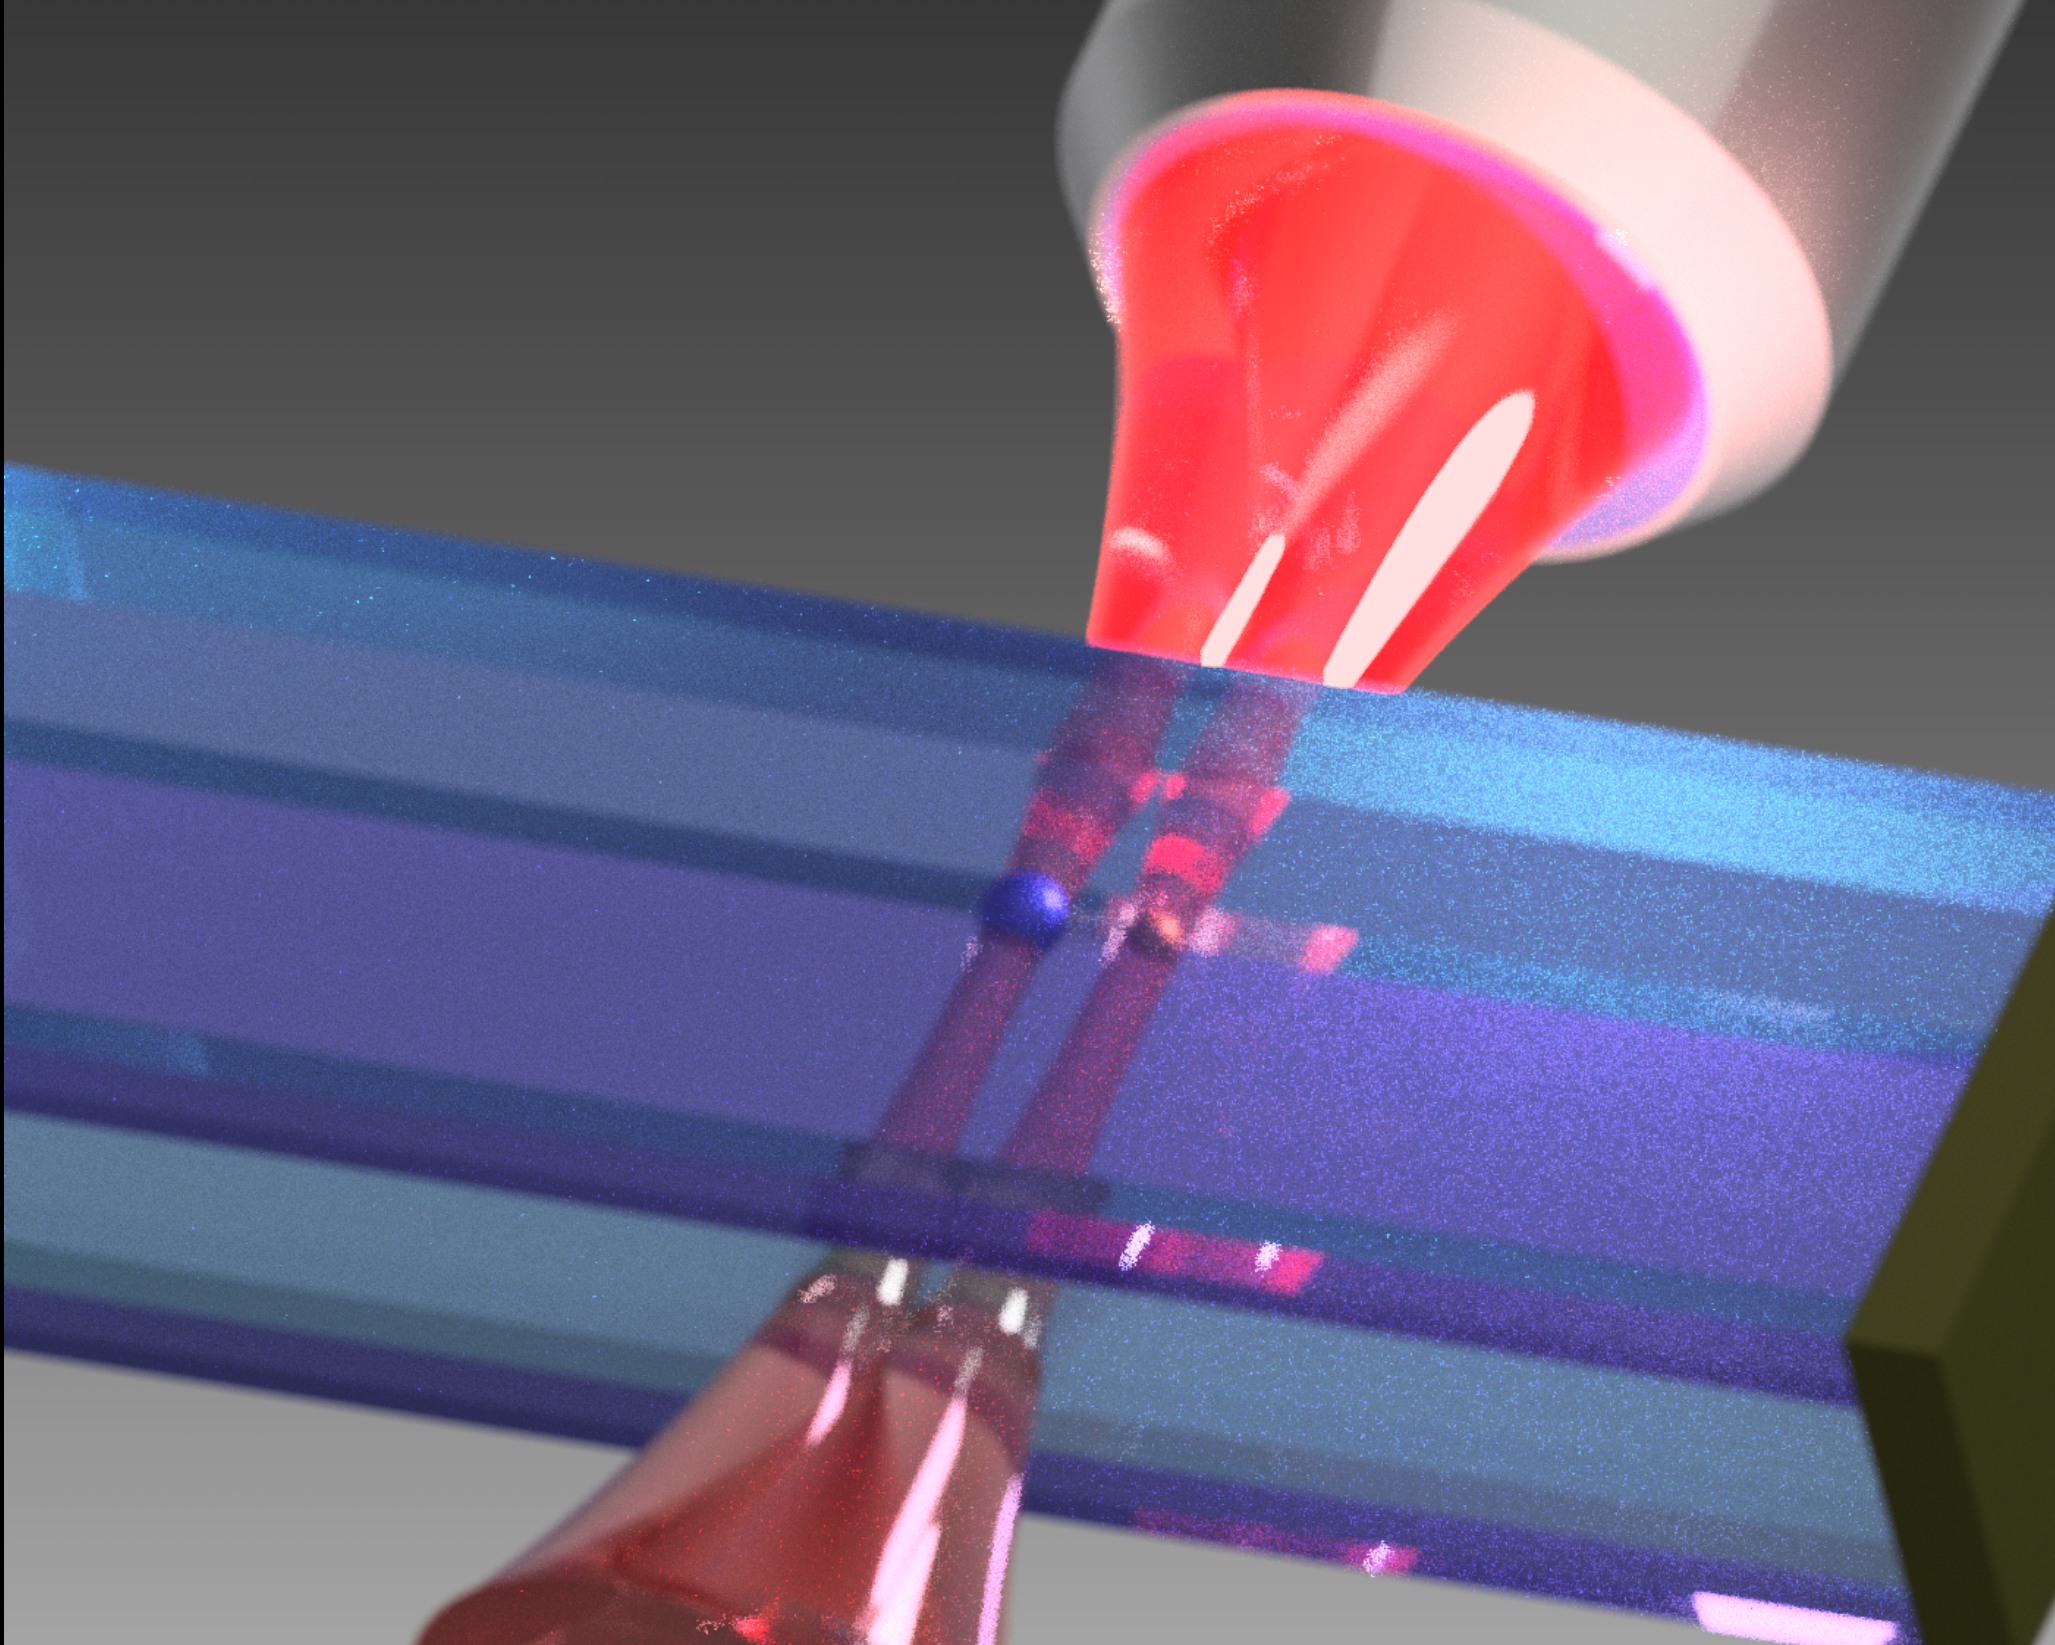
\includegraphics[width=\paperwidth]{front_bg.png}}
  }
  \setbeamercolor{title}{fg=white}
  \setbeamercolor{author}{fg=white}
  \setbeamercolor{institute}{fg=white}
  \setbeamercolor{date}{fg=white}
  \begin{frame}{}
    \titlepage
  \end{frame}
}

%% Goal
% The long term goal of our experiment is to create a new system
% for quantum computing and quantum simulation, as well as, in general,
% adding new tools to the so-called AMO toolbox for potentially other applications.
% These applications require our system to be fully controllable to single particle level
% as well as allowing creating entanglement between the particles.

% There are many good candidates, and even just in AMO there are
% neutral atoms, ions, Rydbergs etc, so why are we adding yet another one to the list.
% Well, first of all, broadly speaking, you'll never know what you'll get unless you try it.
% There are often pleasant supprises, even from the difficulties one face in the experiment,
% as you'll see later.
% (And this really applies to many other things including some big discovery as well.)
% More concretely, although some approaches have got closer to the goal then others,
% no one have actually got there yet and there are still big challeges for all of them.
% So the door is still open, and although I'm definately not going to claim we have the
% best system in the world, I do believe we are bringing in new ideas and
% new solutions for some of the issues in other systems.
\begin{frame}{}
  \begin{center}
    \begin{tikzpicture}
      \node[right, align=center] at (0.7, -1.7) {
        \usebeamercolor[fg]{frametitle}{\small Precision Measurement}\\
        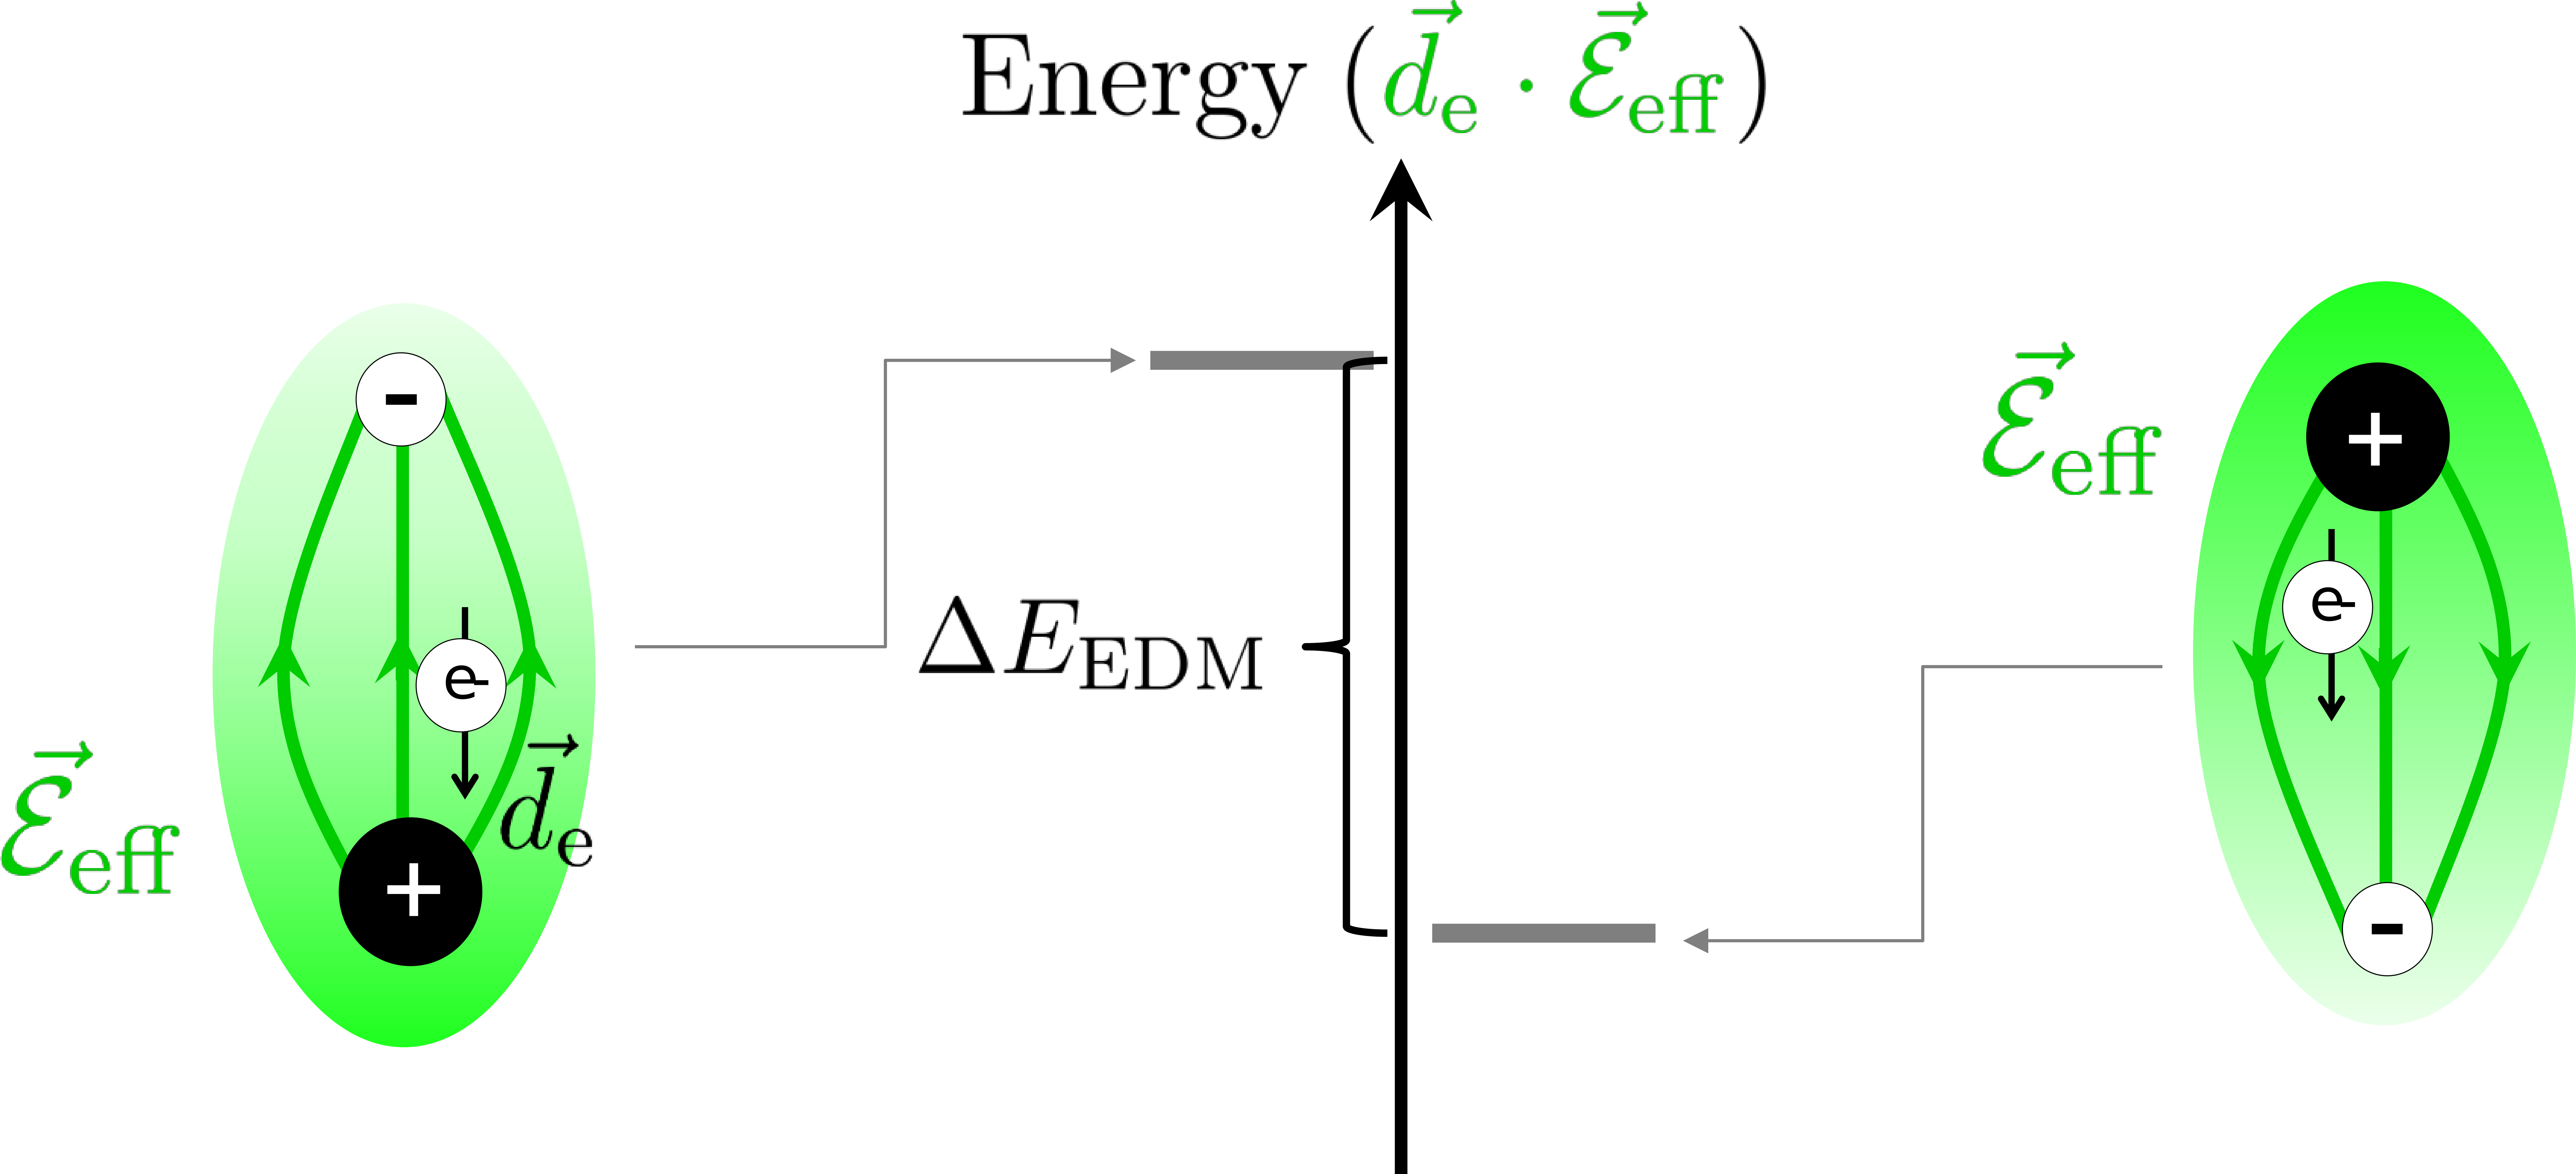
\includegraphics[width=3.2cm]{edm}\\
        {\tiny Science 343, p. 269-272 (2014)}};
      \node[right, align=center] at (4.5, -2.0) {
        \usebeamercolor[fg]{frametitle}{\small Quantum Chemistry}\\
        \includegraphics[width=2.0cm]{quantum_chemistry}\\
        {\tiny Nature 464, 1324 (2010)}};
      \fill[white,opacity=0.4] (8.0, -3.75) rectangle (0.7, -0.1);
      \node[right, align=center] at (1.0, 1.9) {
        \usebeamercolor[fg]{frametitle}{\small Quantum Simulation}\\
        \includegraphics[width=2.9cm]{quantum_simulation}\\
        {\tiny Nat. Phys. 2, 341 (2006)}};
      \node[right, align=center] at (4.2, 2.0) {
        \usebeamercolor[fg]{frametitle}{\small Quantum Computing}\\
        \includegraphics[width=2.9cm]{quantum_computing}\\
        {\tiny PRL. 97, 33003 (2006)}};
      \visible<2->{
        \node[above,text width=4.5cm] at (10, 1) {
          \begin{itemize}
          \item Full quantum control
          \item Entanglement
          \item $\cdots$
          \end{itemize}
        };
      }
      \visible<3->{
        \node[below] at (10, -1.2) {
          \usebeamercolor[fg]{frametitle}
          {\large\textbf{\phantom{\only<3>{?}\only<4->{!}}New Approach\only<3>{?}\only<4->{!}}}
        };
      }
    \end{tikzpicture}
  \end{center}
\end{frame}

%% System
% Hopefully it make sense now that despite all the achievements in other approaches,
% it is still interesting to study new systems, if it has new desired properties.
% So now let's look at our system.

% The two properties that I've emphasized on initially are full quantum control and
% entanglement. And let's first talk about entanglement.
% Well, entangling different particles essentially means interaction.
% And this is the main reason we chose dipole molecules.
% Compared to neutral atoms, they have much stronger and longer range interactions,
% roughly `kHz` about a micron apart. This might not seem like much compared to other strongly
% interacting systems like ions and Rydberg atoms, the interacting molecular
% states are long lived and easily tunable, which is useful for reducing coupling with
% the enviroment and achieve long coherence time.
% Molecules also have a very rich internal state, which is the main reason for the tunability,
% but it also give us a lot of freedom in selection our qubit states, for example.

% The other important property we are aiming for is full quantum control,
% and for that our main tool is the optical tweezer.
% Since the tweezer is generally form through a high-NA objective,
% it very naturally gives us the resolution for single site detection and even manipulation
% of the molecules. This technique has been developped in many other groups for atoms including
% here in Cindy's lab, demostrating sideband cooling, near deterministic loading
% and rearranging.
% So we would like to extend these capability from atoms to molecules and
% you'll see later in my talk how we use this to achieve quantum control on our molcules.
\begin{frame}{}
  \begin{center}
    \begin{tikzpicture}
      \uncover<-8>{
        \node[below,align=center] at (-3, 4) {
          {\usebeamercolor[fg]{frametitle}{\large \textbf{Entanglement}}}\\
          {\visible<2->{
              \usebeamercolor[fg]{frametitle}{\footnotesize \textbf{i.e. interaction}}
            }}
        };
      }
      \visible<3->{
        \node[below,align=center,text width=5.8cm] at (-3, 2.7) {{
            {\uncover<-8>{\usebeamercolor[fg]{frametitle}{\textbf{Dipolar molecules}}}}
            \visible<4-8>{
              \begin{itemize}
              \item Strong and tunable interaction\\
                ($\approx kHz$ at $\approx\mu m$ distance)\\
                \uncover<5->{
                  \begin{itemize}
                  \item Fast gate operations
                  \item Long coherence time
                  \end{itemize}
                }
              \item<6-> Rich internal structure\\
                (Electronic, vibrational, rotational, hyperfine, etc.)
              \end{itemize}
            }
          }};
      }
      \uncover<1,7-> {
        \node[below,align=center] at (3, 4) {
          \usebeamercolor[fg]{frametitle}{\textbf{Single particle control}}};
      }
      \visible<7->{
        \node[below,align=center,text width=5.8cm] at (3, 3) {{
            {\usebeamercolor[fg]{frametitle}{\textbf{Optical tweezers}}}
            \visible<8->{
              \begin{itemize}
              \item Single site resolution
              \item<9-> $\cdots$
              \end{itemize}
            }
          }};
      }
      \visible<9->{
        \node[align=center] at (-3.3, -1.5) {
          \usebeamercolor[fg]{frametitle}{\footnotesize Loading}\\
          \includegraphics[width=3.8cm]{deterministic-loading}\\
          {\tiny Nat. Phys. 6, 951 (2010)}
        };
        \node[align=center] at (2.7, 0) {
          \usebeamercolor[fg]{frametitle}{\footnotesize Cooling}\\
          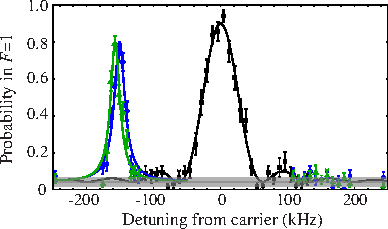
\includegraphics[width=3.5cm]{rsc-regal}\\
          {\tiny PRX. 2, 041014 (2012)}
        };
        \node[align=center] at (2.4, -3.3) {
          \usebeamercolor[fg]{frametitle}{\footnotesize Rearranging}\\
          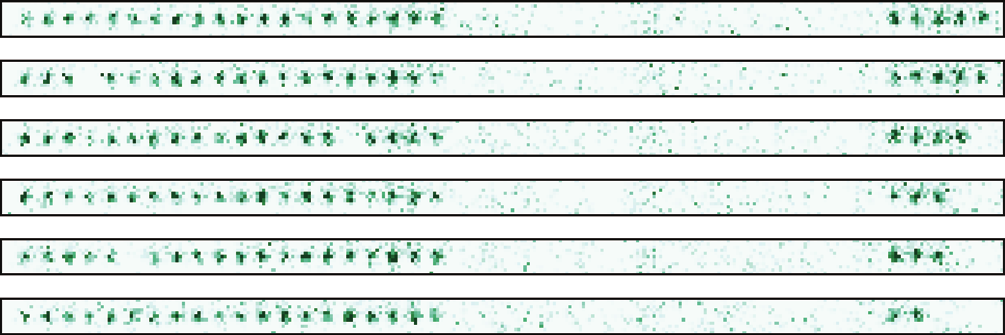
\includegraphics[width=5.7cm]{atom-array}\\
          {\tiny Science 354, 1024 (2016)}
        };
      }
    \end{tikzpicture}
  \end{center}
\end{frame}

%% Molecules in tweezers
% So since our goal is to create ultracold molecules, there are basically two approaches.
% One approach is to first get molecule and then get ultracold, in another word, direct cooling
% of hot molecules to ultracold temperature without destroying or otherwise loosing the molecule.
% This is a very hard problem because of the difficulties in laser cooling, but there
% has been a lot of progress in this area, including an experiment here at JILA in Jun's group.
% In fact, the Doyle group at Harvard have recently demostrated ultracold CaF molecules
% in an array of optical tweezers, as you can see in this picture.

% The other approach, which is what we use, is to get ultracold, and then get molecule.
% In another word, we would cool and fully control whatever make up the molecule,
% in our case atoms, before turning them into molecule coherently,
% without heating them, and in general maintaining the control we had on them in this process.

% Comparing the two approaches, the main challenge currently for the direct cooling approach
% is to cool and in general controlling the molecules in the tweezer. Whereas for us,
% our challenge is to first obtaining the control on the atom, and the coherence creation of the
% molecules. These two main challenges will be what I'm going to focus on
% for the remainder of my talk.
% <6min>
\begin{frame}{Ultracold molecule in tweezers}
  \begin{center}
    \begin{tikzpicture}
      \node at (-3, 4) {\usebeamercolor[fg]{frametitle}{\textbf{Direct cooling}}};
      \node[below, align=center] at (-3, 3.5) {
        \includegraphics[width=6cm]{CaF_tweezer.png}\\
        \vspace{0.5cm}
        \scriptsize Science 365, 1156 (2019)
      };

      \visible<2->{
        \node at (3, 4) {\usebeamercolor[fg]{frametitle}{\textbf{Assembly}}};
        \begin{scope}[shift={(1.6, 3.2)}, scale=0.5]
          \shade[ball color=blue!90] (-0.8, 0.2) circle (0.45);
          \shade[ball color=orange!90] (0.3, -0.2) circle (0.3);
        \end{scope}
        \node[align=center] (atom) at (3, 3.2) {\hspace{1cm}\textbf{Ultracold atoms}};
        \begin{scope}[shift={(1.35, 1.5)}, scale=0.5]
          \shade[ball color=blue!90] (-0.2, -0.1) circle (0.45);
          \shade[ball color=orange!90] (0.2, 0.1) circle (0.3);
        \end{scope}
        \node[align=center] (molecule) at (3, 1.5) {\hspace{1cm}\textbf{Ultracold molecule}};
        \draw[blue, ->, line width=2] (atom) --
        node[right] {\small \textbf{Coherent transfer}} (molecule);
      }

      \visible<3->{
        \node at (0, 0) {\usebeamercolor[fg]{frametitle}{\underline{\textbf{Challenges}}}};
      }

      \visible<3->{
        \node[below, text width=5.5cm, align=left] at (-3, -0.8) {\begin{itemize}
          \item Temperature in tweezer
          \item Quantum control
          \end{itemize}};
      }

      \visible<4->{
        \node[below, text width=4cm, align=left] at (3, -0.7) {\begin{itemize}
          \item Creating molecules
          \item Maintain coherence
          \end{itemize}};
      }
    \end{tikzpicture}
  \end{center}
\end{frame}

% So here's an outline for the rest of my talk.
% I'll first give an overview of our experiment, both the procedure and the apparatus.
% Then I'll discuss about one example of achieving full control on our atoms.
% And after that I'll talk about how we create the molecule while maintaining this
% control, before giving my conclusion.
\begin{frame}{Outline}
  \tableofcontents
\end{frame}

\section{Experiment overview}
% So first the experiment.
% The molecules we make is NaCs, chosen because
% a) the alkali atoms are relatively easy to cool and control, and
% b) this molecule has a fairly strong dipole moment of 4.6 debye among the bi-alkalis.

% Since we are making molecules from atoms inside the optical tweezer,
% the obvious first step is to get the atoms in there.
% We trap the atoms in their respective tweezers directly from the MOT as you can see
% in this picture, with abouot 60% loading probability.

% We then prepare the initial state, both internal and motional,
% for the atoms using optical pumping and Raman sideband cooling to a single state
% with a fairly high fidelity, which I'll talk about later.

% At this point the atoms are still in their own tweezers,
% which isn't very helpful for making a single molecule.
% So the natural next step is to move one of the tweezers and
% merge the two atoms into the same tweezer.
% We do this in a way that minimize the heating to the two atoms so they remain in their
% motional ground states that we cooled them into.

% After the merge, the two atoms are now in the same trap and
% we proceed to form the molecule from this state.
\begin{frame}[t]{Experiment overview}
  \vspace{-0.5cm}
  \begin{center}
    \begin{tikzpicture}[scale=0.7]
      \mytweezer.drawCsTweezer(0, 0)
      \mytweezer.drawNaTweezer(-1, 0)
      \mytweezer.drawCsAtom(-0.07, 0.08, 0.22)
      \mytweezer.drawNaAtom(-1.06, -0.09, 0.27)

      \mytweezer.drawCsTweezer(0, -3.1)
      \mytweezer.drawNaTweezer(-1, -3.1)
      \mytweezer.drawCsAtom(0.0, -3.1, 0.12)
      \mytweezer.drawNaAtom(-1.0, -3.1, 0.16)

      \mytweezer.drawCsTweezer(-1, -7.0)
      \mytweezer.drawNaAtom(-1.05, -6.87, 0.16)
      \mytweezer.drawCsAtom(-0.95, -7.13, 0.12)

      \fill[white,temporal=<1>{opacity=0.82}{opacity=0}{opacity=0.5}]
      (-1.5, 1.5) rectangle (0.5, -1.5);
      \fill[white,temporal=<2>{opacity=0.82}{opacity=0}{opacity=0.5}]
      (-1.5, 1.5 - 3.1) rectangle (0.5, -1.5 - 3.1);
      \fill[white,temporal=<3>{opacity=0.82}{opacity=0}{opacity=0.5}]
      (-1.5, 1.5 - 7.0) rectangle (-0.5, -1.5 - 7.0);

      \visible<2->{
        \begin{scope}[alt=<2>{opacity=0.7}{opacity=0.35}]
          \draw[orange,dotted,line width=1.2] (-1, -0.4) -- (-1, -2.9);
          \draw[blue,dotted,line width=1.2] (0, -0.15) -- (0, -2.9);
        \end{scope}
      }

      \visible<3->{
        \begin{scope}[alt=<3>{opacity=0.7}{opacity=0.35}]
          \draw[->,orange,line width=1.2] (-1, -3.3) -- (-1, -6.7);
          \draw[->,blue,domain=-3.3:-6.7,smooth,variable=\y,line width=1.2]
          plot ({atan((\y+4.7) * 5) / 170 - 0.5},{\y});
        \end{scope}
      }
      \visible<1>{
        \node[above,align=center] at (7, 0)
        {\usebeamerfont{frametitle}\usebeamercolor[fg]{frametitle}{\Large Loading}};
        \node[below,align=center] at (6.5, -0.5)
        {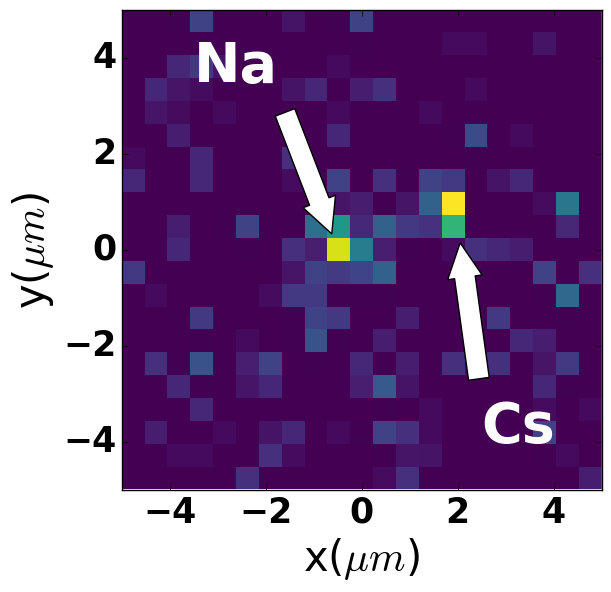
\includegraphics[width=5cm]{../../experiments/nacs_atoms/imgs/single_viridis.png}};
        \node[below,align=center] at (7, -7.5)
        {Loading probability per site: 60\%\\
          Post select on initial and final state.};
      }
      \visible<2>{
        \node[above,align=center] at (7, 0)
        {\usebeamerfont{frametitle}\usebeamercolor[fg]{frametitle}{\Large Cooling}};
        \node[below] at (6.5, -1)
        {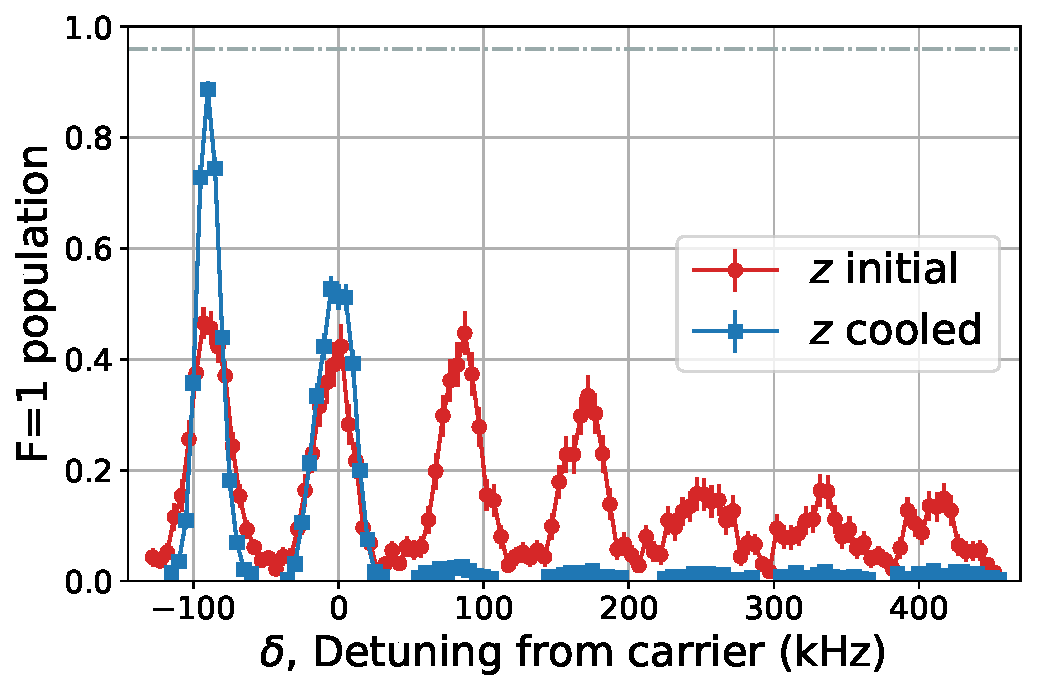
\includegraphics[width=6cm]{spectrum_nolabel_az.pdf}};
        Don't mention axis.
        Explain the sideband spectrum more.
        \only<2>{
          \node[below,align=center] at (7, -7)
          {Cs: 96\% ground state\footnote{Phys. Rev. X 9, 021039}\\
            Na: 94\% ground state\footnote{Phys. Rev. A 97, 063423}};
        }
      }
      \visible<3>{
        \node[above,align=center] at (7, 0)
        {\usebeamerfont{frametitle}\usebeamercolor[fg]{frametitle}{\Large Merging}};
        \draw[orange,line width=1.5] plot[draw,samples=200,domain=4.5:10.5]
        function {-0.22 * exp(-(x - 9)**2 / 0.75**2) + -0.4 * exp(-(x - 6)**2 / 0.75**2) - 1};
        \draw[blue,line width=1.5] plot[draw,samples=200,domain=4.5:10.5]
        function {-1.2 * exp(-(x - 9)**2 / 0.75**2) + 0.45 * exp(-(x - 6)**2 / 0.75**2) - 1};
        \mytweezer.drawNaAtom(6, -1.22, 0.15)
        \mytweezer.drawCsAtom(9, -2.06, 0.11)

        \draw[orange,line width=1.5] plot[draw,samples=200,domain=4.5:10]
        function {-0.22 * exp(-(x - 7.5)**2 / 0.75**2) + -0.4 * exp(-(x - 6)**2 / 0.75**2) - 3.5};
        \draw[blue,line width=1.5] plot[draw,samples=200,domain=4.5:10]
        function {-1.2 * exp(-(x - 7.5)**2 / 0.75**2) + 0.45 * exp(-(x - 6)**2 / 0.75**2) - 3.5};
        \mytweezer.drawNaAtom(6, -3.72, 0.15)
        \mytweezer.drawCsAtom(7.5, -4.56, 0.11)

        \draw[orange,line width=1.5] plot[draw,samples=200,domain=4.5:8.5]
        function {-0.22 * exp(-(x - 6)**2 / 0.75**2) + -0.4 * exp(-(x - 6)**2 / 0.75**2) - 6};
        \draw[blue,line width=1.5] plot[draw,samples=200,domain=4.5:8.5]
        function {-1.2 * exp(-(x - 6)**2 / 0.75**2) + 0.45 * exp(-(x - 6)**2 / 0.75**2) - 6};
        \mytweezer.drawNaAtom(5.9, -6.42, 0.12)
        \mytweezer.drawCsAtom(6.05, -6.6, 0.13)

        \draw[orange,line width=1.5] plot[draw,samples=200,domain=4.5:8.5]
        function {-0.22 * exp(-(x - 6)**2 / 0.75**2) - 8.5};
        \draw[blue,line width=1.5] plot[draw,samples=200,domain=4.5:8.5]
        function {-1.2 * exp(-(x - 6)**2 / 0.75**2) - 8.5};
        \mytweezer.drawNaAtom(6, -8.55, 0.14)
        \mytweezer.drawCsAtom(6, -9.56, 0.11)

        \draw[dotted,line width=2,black!30,opacity=10] (0.3, -3.0) -- (4.5, -0.5);
        \draw[dotted,line width=2,black!30,opacity=10] (-0.7, -7.0) -- (4.5, -9.3);
      }
    \end{tikzpicture}
    \vspace{-2cm}
  \end{center}
\end{frame}

%% Lab pictures
% In real world this experiment looks like this.
% Since we don't need to trap a lot of atoms and we also don't use any rediculously strong field,
% our experiment is relatively small and compact.
% You can see in this picture our whole vacuum chamber with the optics surounding it
% for cooling, detection, etc.
% It might not look too impressive compared to an ion experiment,
% I know some of those are real neat, but it's already very clean compared to
% some other neutral atom experiments that I've worked on before...
% <10min>
\begin{frame}{}
  \begin{center}
    \begin{tikzpicture}
      \visible<1>{
        \node at (-3, 0) {\includegraphics[width=9cm]{chamber}};
      }
      \visible<2-3>{
        \node at (-3, 0) {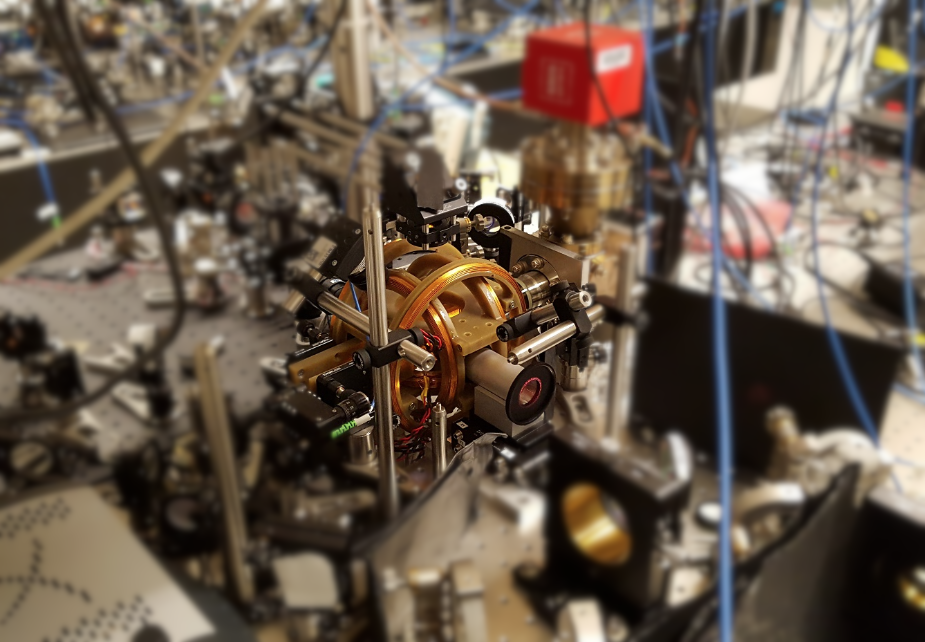
\includegraphics[width=9cm]{chamber_center}};
      }
      \visible<4>{
        \node at (-3, 3.5) {\usebeamercolor[fg]{frametitle}{\textbf{MOT beam path}}};
        \node at (-3, 0) {\includegraphics[width=9cm]{chamber_mot}};
      }
      \visible<5>{
        \node at (-3, 3.5) {\usebeamercolor[fg]{frametitle}{\textbf{Tweezer beam path}}};
        \node at (-3, 0) {\includegraphics[width=9cm]{chamber_tweezer}};
      }
      \visible<3> {
        \draw[white, line width=2] (-3.1, -0.2) ellipse (0.25 and 0.4);
        \draw[white, line width=1.5] (-3.15, 0.2) -- (-0.5, 1.65);
        \draw[white, line width=1.5] (-3.15, -0.6) -- (-0.5, -1.65);
        \draw[white, line width=3] (-0.5, 1.65) rectangle (4.5, -1.65);
        \node at (2, 0) {\includegraphics[width=5cm]{na_mot}};
        \fill[black, opacity = 0.3, even odd rule]
        (-0.5, 1.65) rectangle (4.5, -1.65) (1.9, 0.35) circle (0.3);
        \node[below, white] at (1.9, -0.1) {\textbf{\small Na MOT}};
      }
    \end{tikzpicture}
  \end{center}
\end{frame}

%% Atom control
% So next I'll talk about our state control of the atom.
% Of course, even for atoms, there are many degrees of freedoms to control
% and I don't have time to talk about every single one of them.
% So instead, I'm just going to focus on how we use Raman sideband cooling to cool Na atoms.
\section{Atom state control}
\subsection{Raman sideband cooling of Na atoms}
\begin{frame}{Outline}
  \tableofcontents[currentsection,currentsubsection]
\end{frame}

%% Raman sideband cooling
% I imagine most people here are very familiar with Raman sideband cooling.
% In fact, I feel like it is used so common in ion experiments that people stops
% talking about it. So I believe I don't have to talk too much about how it works in general.
% Instead, I'll focus on the difference in our experiment and the new challenges we face.
% And I'll talk about how we overcome these challenges and open up this tool to
% ours and other future experiments where Raman sideband cooling were previously thought
% to be very hard or impossible.

% Before that, let me just very quickly go through how Raman sideband cooling works
% even though you probably know already.
% So here is the motional levels of an atom in a harmonic potential, which approximate our
% optical tweezer. These levels exists for all the ground HF states so here is it for a different
% one. Now, we can drive between different ground HF states with a Raman transitions.
% But due to the motional levels, in additional to driving a "carrier" Raman transition,
% we can also drive "sideband" transitions that changes the motional state
% in additional to the HF states.
% Now, if we drive such a transition that removes a quanta of motional energy from the
% atom, followed by an optical pumping step that removes the emtropy and
% resets the HF state of the atom,
% we would have overall reduced the motional energy of the atom, therefore cooling it.
\begin{frame}{Raman sideband cooling}
  % TODO
\end{frame}

% Lamb-Dicke parameter
% It is not too hard to see that whether this cooling cycle can work relies on the balance
% between removing motional energy from the atom via the sideband transition,
% and the heating done in the OP step. This ratio is determined by the so-called Lamb-Dicke
% parameter, which is defined as the ratio between the harmonic oscillator length
% and the Raman or OP wavelengths, and it is also proportional to the square root of the
% recoil energy and the trapping frequency, which is exactly what we want.
% Because of this, one would like a small LD parameter so that the heating is small
% compared to the cooling. This is OK for Cs and also for Rb which was demostrated
% in other groups before, but the light mass of Na as well as the short wavelength
% of the D lines causes a much bigger LD parameter.
% Together with a higher initial temperature for Na due to lack of good PGC,
% we knew right off the bat that Na cooling will be hard.
% But still, the LD parameter is smaller than one so we decided to give it a try
% and it turns out that the difficulty with RSC for Na is more subtle then what one
% might naively expect.

% First of all, although the Lamb-Dicke parameter tells us that we should have
% a net cooling per cycle on average, it does not capture the uncertainty of cooling process
% as you can see in this plot, with a high Lamb-Dicke parameter, the atom might end up
% in a wide varity of states and it is worse the high the initial state is.
% Second, which is makes the first issue worse, is the variation of the coupling.
% The sideband coupling for different motional states are different. This is not news
% for people doing sideband cooling and in fact we leart from Till Roseband to take this
% into account for our Cs RSC based on his old experience with RSC on ions right here at NIST.
% However, what's new for Na is that our Lamb-Dicke parameter and initial tempereture is high
% enough that we are experiencing coupling "dead zone"s.
% If the atoms gets here, we would not be able to address them as efficiently
% (and can't be easily fixed by changing the pulse times) and they also won't show up
% in our detection making optimization very hard.

% The solution we found to these problem turns out to be the large Lamb-Dicke parameter itself.
% You see, the fact that a large Lamb-Dicke parameter cause more heating
% and more spread out of states actually also means that the atoms has a strong coupling
% to higher order sideband. Now if we use these higher order sideband to do the cooling
% we can significantly increase the cooling to heating ratio, fixing the original concern
% for RSC. It doesn't directly fix the spreading out problem but it does give us
% more ways to deal with it.
% Most importantly though, if we add higher order sideband to this plot for the coupling strength
% we can see that the dead zone is completely gone. Depending on which states we want to cool,
% we can now simply pick the sideband order where the coupling is the largest
% and we'll be able to cool them down.

% With the additional complexity of the higher orders, we switched to a computer simulation
% to guide our search so that we don't have to interpret the signal for
% many different sideband orders. We use it to test different experimental sequences
% and come up with this sequence that always address two neighboring orders of sideband.
% When we implemented it in the experiment after calibration all the parameters, this
% is the result we got. We have very clear suppression of the cooling sideband
% and this result suggests that we have a 94% ground state population for Na,
% despite a high Lamb-Dicke parameter and initial temperature.
\begin{frame}{}
  % TODO
\end{frame}

% TODO?
% \subsection{Interaction shift}
% \begin{frame}{Outline}
%   \tableofcontents[currentsection,currentsubsection]
% \end{frame}

\section{Optical molecule creation}
% So now we've overcame one of the last and biggest challenge we had
% on preparing the initial state for the atom. I'll now talk about how we
% make the molecules while maintaining this control.
\begin{frame}{Outline}
  \tableofcontents[currentsection]
\end{frame}

%% Size mismatch/optical transfer
% So here's a summary of our control of the atom.
% After we merge the two atoms into the same tweezer,
% the two atoms are about as closed to each other as they can be
% from the confinement. However, in the molecule we want to make,
% the two atoms are still hundreds times closer.
% This massive size mismatch is really the biggest challange for creating molecules coherently.
\begin{frame}{}
  \begin{center}
    \begin{tikzpicture}
      \node[below,align=center] at (1.75, 4)
      {\hspace{0.5cm}\usebeamerfont{frametitle}\usebeamercolor[fg]{frametitle}{Loading}\\
        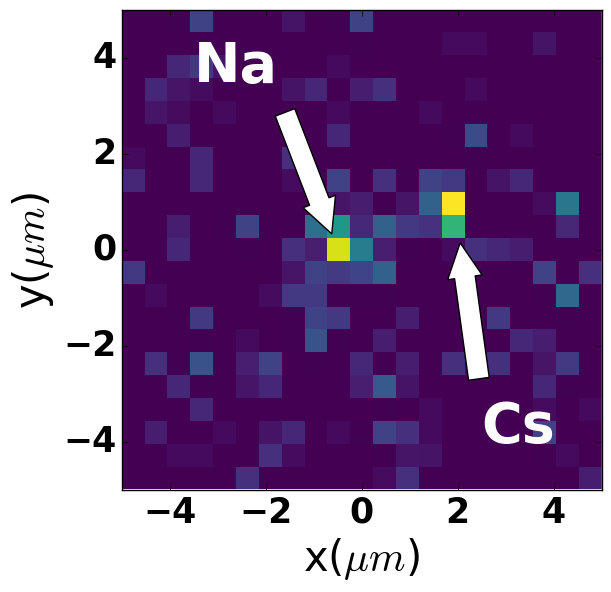
\includegraphics[width=3cm]{../../experiments/nacs_atoms/imgs/single_viridis.png}};
      \node[above,align=center] at (2, 0.36)
      {\usebeamercolor[fg]{frametitle}{\tiny{NJP. 19, 023007 (2017)}}};
      \node[below,align=center] at (2.1, 0.28)
      {\usebeamerfont{frametitle}\usebeamercolor[fg]{frametitle}{Cooling}\\
        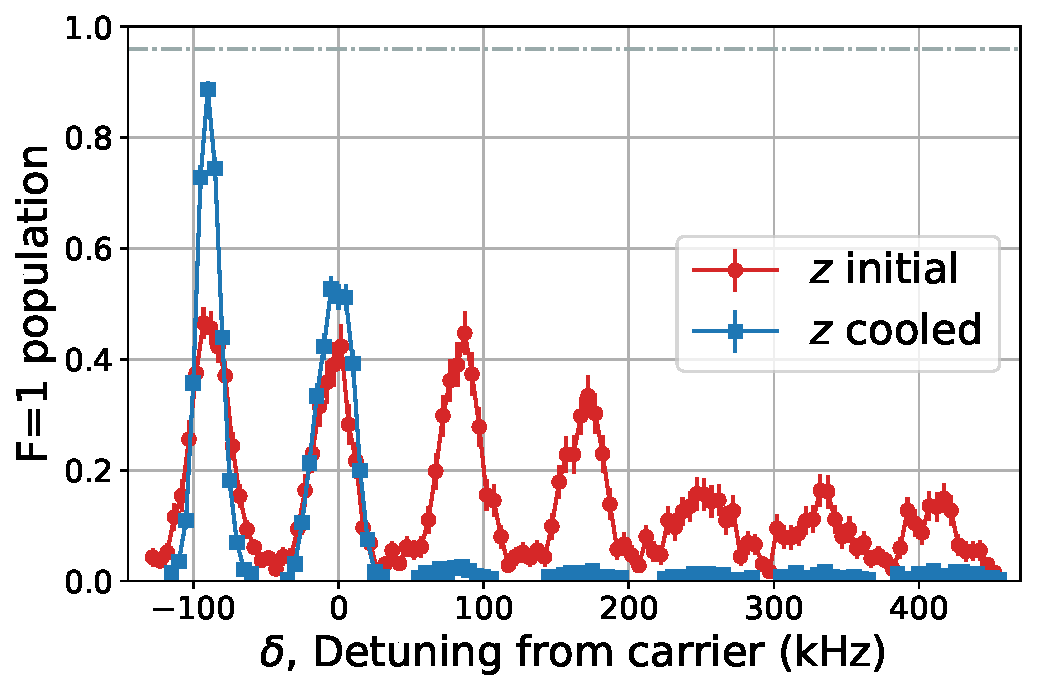
\includegraphics[width=4.2cm]{spectrum_nolabel_az.pdf}};
      \node[below,align=center] at (5.25, 3.5)
      {\usebeamerfont{frametitle}\usebeamercolor[fg]{frametitle}{Merging}};
      \node[above,align=center] at (2.2, -3.3)
      {\usebeamercolor[fg]{frametitle}{\tiny{PRA. 97, 063423 (2018)}}};
      \node[above,align=center] at (5.4, -3.1)
      {\usebeamercolor[fg]{frametitle}{\tiny{PRX. 9, 021039 (2019)}}};
      \begin{scope}[shift={(4.8, 4)}, xscale=-0.8, yscale=0.8]
        \mytweezer.drawCsTweezer(0, -3.1)
        \mytweezer.drawNaTweezer(-1, -3.1)
        \mytweezer.drawCsAtom(0.0, -3.1, 0.12)
        \mytweezer.drawNaAtom(-1.0, -3.1, 0.16)

        \mytweezer.drawCsTweezer(-1, -7.0)
        \mytweezer.drawNaAtom(-1.05, -6.87, 0.16)
        \mytweezer.drawCsAtom(-0.95, -7.13, 0.12)

        \begin{scope}[opacity=0.7]
          \draw[->,orange,line width=1.2] (-1, -3.3) -- (-1, -6.7);
          \draw[->,blue,domain=-3.3:-6.7,smooth,variable=\y,line width=1.2]
          plot ({atan((\y+4.7) * 5) / 170 - 0.5},{\y});
        \end{scope}
      \end{scope}
      \visible<2->{
        \begin{scope}[shift={(9.5, 2.5)}, scale=0.8]
          \draw[line width=1] plot[samples=200,domain=-2:2,variable=\x] ({\x + 0}, {(\x)^2 * 0.8 - 1.5});
          \draw[line width=2,orange!90!black]
          plot[samples=200,domain=-2:2,variable=\x] ({\x + 0}, {exp(-(\x)^2 * 1.3) - 0.988});
          \draw[line width=0.8] (0 - 0.8, -0.988) -- (0 + 0.8, -0.988);
          \draw[<->,line width=1] (0 - 1, 0.3) -- (0 + 1, 0.3);
          \path (0, 0.3) node[above] {$1000a_0$};
          \path (0, -1.8) node[below] {\textbf{Atom}};
        \end{scope}
        \begin{scope}[shift={(9.5, -1.5)}, scale=0.8]
          \shade[ball color=blue!90] (0, 0) circle (0.45);
          \shade[ball color=orange!90] (0.4, 0.2) circle (0.3);
          \draw[<->,line width=1] (-0.45, 0.4) -- (0.35, 0.8);
          \path (-0.05, 0.6) node[rotate=26.565,above=2pt] {$4a_0$};
          \path (0, -1) node[below] {\textbf{Molecule}};
        \end{scope}
      }
    \end{tikzpicture}
  \end{center}
\end{frame}

%% Size mismatch
% ... which basically necessitate a two step transfer process.
% The more loosely bound intermediate molecular state reduces
% the size mismatch and will improve overall efficiency.
% In today's talk, I'll mostly focus on the first step starting from the atomic state
% (as you might have guessed from the title of my talk).

% The "tranditional" choice of the intermediate state is a FB molecule.
% Indeed, it also works for us and we've recently created a single FB
% molecule in the optical tweezer that is suitable for doing the next step transfer from.
% However, this approach obviously rely on finding a good FB resonance and usually
% a large magentic field.

% What I am going to talk about today, OTOH, is a different approach that uses only
% optical transitions. By not relying on FB resonance, it is faster, more compact,
% and most importantly, we hope it can be more generally apply to
% molecules that may not have a suitable FB resonance.

% It's worth pointing out that optical transfer **has** been done previously
% on many systems include this Rb2 Raman resonance and even a previous attempt from our lab.
% However, it was either done incoherently, or it relies on narrow line transition
% which limits the generality of the result.
% So next I'll talk about how we overcome these limitations.

\begin{frame}{}
  \begin{center}
    \begin{tikzpicture}
      \begin{scope}[shift={(-1, 0)}, scale=0.9]
        \begin{scope}[shift={(-5, 3)}, scale=0.6]
          \draw[line width=1] plot[samples=200,domain=-2:2,variable=\x] ({\x + 0}, {(\x)^2 * 0.8 - 1.5});
          \draw[line width=2,orange!90!black]
          plot[samples=200,domain=-2:2,variable=\x] ({\x + 0}, {exp(-(\x)^2 * 1.3) - 0.988});
          \draw[line width=0.8] (0 - 0.8, -0.988) -- (0 + 0.8, -0.988);
          \draw[<->,line width=1] (0 - 1, 0.3) -- (0 + 1, 0.3);
          \path (0, 0.3) node[above] {$1000a_0$};
          \path (0, -1.8) node[below] {\small \textbf{Atom}};
        \end{scope}
        \begin{scope}[shift={(-2.2, 3)}, scale=0.6]
          \shade[ball color=blue!90] (-0.4, -0.1) circle (0.55);
          \shade[ball color=orange!90] (0.4, 0.3) circle (0.4);
          \draw[<->,line width=1] (-1.05, 0.4) -- (0.55, 1.2);
          \path (-0.25, 0.8) node[rotate=26.565,above=2pt] {$\approx 20\!-\!200a_0$};
          \path (0, -1.2) node[below,align=center] {\small \textbf{Weakly-Bound}\\\small \textbf{Molecule}};
        \end{scope}
        \begin{scope}[shift={(0, 3)}, scale=0.6]
          \shade[ball color=blue!90] (0, 0) circle (0.45);
          \shade[ball color=orange!90] (0.4, 0.2) circle (0.3);
          \draw[<->,line width=1] (-0.45, 0.4) -- (0.35, 0.8);
          \path (-0.05, 0.6) node[rotate=26.565,above=2pt] {$4a_0$};
          \path (0, -1) node[below] {\small \textbf{Molecule}};
        \end{scope}
        \visible<2->{
          \draw[line width=1, red] (-6.4, 4.35) rectangle (-0.9, 1.35);
        }
      \end{scope}
      \visible<3-4>{
        \node at (-3, 0.8) {\usebeamercolor[fg]{frametitle}{\textbf{Feshbach molecule}}};
        \node[below, align=center] at (-3.2, 0.4)
        {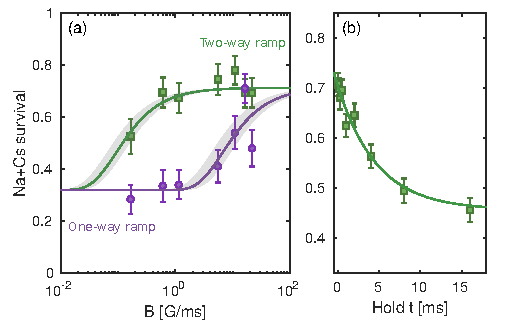
\includegraphics[width=6cm]{fb_molecules.pdf}\\
          \small{PRL. 124, 253401 (2020)}};
        \visible<4->{
          \node[below, text width=6cm, align=left] at (3, -0.3) {\begin{itemize}
            \item Requires Feshbach resonance
            \item Usually large magnetic field
            \end{itemize}
          };
        }
      }
      \visible<5->{
        \node[below, text width=6cm, align=center] at (-3.3, 1)
        {{\usebeamercolor[fg]{frametitle}{\textbf{Optical transfer}}}\\
          \begin{itemize}
          \item More general
          \item Faster
          \end{itemize}
        };
      }
      \visible<6->{
        \node[below, text width=6cm, align=left] at (3.1, 4)
        {
          {\usebeamercolor[fg]{frametitle}{Previous results}}\\
          {\footnotesize $\mathrm{Rb_2}$}
          {\tiny \usebeamercolor[fg]{frametitle}{Science 287, p. 1016-1019 (2000)}}\\
          \phantom{{\footnotesize $\mathrm{Rb_2}$}}
          {\tiny \usebeamercolor[fg]{frametitle}{PRL. 93, 073002 (2004)}}\\
          \includegraphics[width=3.5cm]{Rb2_raman.png}\\
          {\footnotesize $\mathrm{Sr_2}$}
          {\usebeamercolor[fg]{frametitle}{\tiny PRL. 109, 115302 (2012)}}\\
          {\footnotesize $\mathrm{NaCs}$}
          {\usebeamercolor[fg]{frametitle}{\tiny PRX. 9, 021039 (2019)}}\\
          \includegraphics[width=3.5cm]{old_raman_transfer.pdf}
        };
      }
      \visible<7->{
        \node[below, text width=6cm, align=center] at (-3.3, -1.3)
        {
          {\usebeamercolor[fg]{frametitle}{Limitations so far}}\\
          \begin{itemize}
          \item Incoherent due to scattering
          \item Rely on narrow line optical transition
          \end{itemize}
        };
      }
    \end{tikzpicture}
  \end{center}
\end{frame}

%% Raman scheme
% The scheme we use is actually very simple.
% We simply drive a Raman transition from the atomic state to the molecular
% state, detuned from some excited molecular state.

% Since one of the major challenges is the mismatch of the wavefunction size,
% it makes sense to pick a molecular state that is as "big" as possible,
% i.e. the molecular states that are closed to the threshold or even the first bound state.
% Indeed, this is what all previous attempts use which leads to a fairly strong Raman transition.
% However, these states are very closely spaced, and in case of the excited state, this makes
% it hard to detune and reduce the scattering, which ultimately limits the coherence,
% as I metioned previously.
% If we instead use an excited state that is more deeply bound.
% Even though the Raman coupling, we can now detune further to reduce the scattering
% without worrying about hitting another state.

% It may not be obvious if the deeply bound state costs too much in the Raman coupling
% compared to the scattering reduction. That's why we did a calculation to compare the two.

% From the two plots for two different excited states,
% you can easily see that the Rabi frequency to scattering ratio, shown in green
% on the right side axis, never reaches higher than ~1.3 for the near threshold state
% whereas for the deeply bound state we can get a ratio north of 50 when a larger
% detuning is used.

\begin{frame}[t]{Raman transfer}
  \begin{center}
    \vspace{-0.9cm}
    \begin{tikzpicture}
      \begin{scope}[scale=0.8]
        \draw[->,line width=1.2] (0, 0) -- (0, 8);
        \node[above,rotate=90] at (0, 4) {Energy};
        \draw[->,line width=1.2] (0, 0) -- (5.4, 0);
        \node[below] at (2.7, -0.1) {Internuclear distance};

        \draw[cyan!85!blue] ({(1.0269 + 0.25) * 0.7}, 2.5) -- (7.25 * 0.7, 2.5);

        \draw[line width=1.1,cyan!85!blue]
        plot[samples=200,domain=0.96:7,variable=\x]
        ({(\x + 0.25) * 0.7}, {(6.8*\x^(-3.4)-6.5*\x^(-1.7)) * 1.3 + 2.5});

        \draw[line width=1.1,red]
        plot[samples=200,domain=1:7.5,variable=\x]
        ({(\x - 0.75) * 0.7}, {(9.2*\x^(-2.5)-9.0*\x^(-1.3)) * 1.3 + 7.5});
        \node[above right,red] at (0.55 * 0.7, 7.2) {$c^3\Sigma^+$};

        \visible<-2,4>{
          \draw[red] ({(1.1102 - 0.75) * 0.7}, -0.69 * 1.3 + 7.5) --
          ({(6.5 - 0.75) * 0.7}, -0.69 * 1.3 + 7.5);
        }
        \visible<3->{
          \draw[red] ({(1.4 - 0.75) * 0.7}, -1.8 * 1.3 + 7.5) --
          ({(2.5 - 0.75) * 0.7}, -1.8 * 1.3 + 7.5);
        }
        \visible<-2>{
          \draw[black!40,dashed,line width=1] ({(0.9 - 0.75) * 0.7}, -0.77 * 1.3 + 7.5) --
          ({(7 - 0.75) * 0.7}, -0.77 * 1.3 + 7.5);
        }
        \visible<3>{
          \draw[black!40,dashed,line width=1] ({(1.2 - 0.75) * 0.7}, -2 * 1.3 + 7.5) --
          ({(3 - 0.75) * 0.7}, -2 * 1.3 + 7.5);
        }
        \visible<4->{
          \draw[blue, line width=1]
          ({(1.1102 - 0.75) * 0.7 - 0.15}, -0.69 * 1.3 + 7.5 - 0.15) rectangle
          ({(6.5 - 0.75) * 0.7 + 0.15}, -0.69 * 1.3 + 7.5 + 0.15);
          \coordinate (ThresholdHighlight)
          at ({(6.5 - 0.75) * 0.7 + 0.25}, -0.69 * 1.3 + 7.5 - 0.08);
          \draw[blue, line width=1]
          ({(1.4 - 0.75) * 0.7 - 0.15}, -1.8 * 1.3 + 7.5 - 0.15) rectangle
          ({(2.5 - 0.75) * 0.7 + 0.15}, -1.8 * 1.3 + 7.5 + 0.15);
          \coordinate (DeepHighlight)
          at ({(2.5 - 0.75) * 0.7 + 0.25}, -1.8 * 1.3 + 7.5);
        }

        \mytweezer.drawNaAtom(6.55 * 0.7, 2.6, 0.12)
        \mytweezer.drawCsAtom(7.05 * 0.7, 2.6, 0.10)

        \draw[cyan!85!blue] ({(1.0793 + 0.25) * 0.7}, -0.28 * 1.3 + 2.5) -- ({(6 + 0.25) * 0.7}, -0.28 * 1.3 + 2.5);
        \mytweezer.drawNaAtom(4.08 * 0.7, -0.19  * 1.3 + 2.5, 0.12)
        \mytweezer.drawCsAtom(4.25 * 0.7, -0.19  * 1.3 + 2.5, 0.10)

        \visible<-2>{
          \draw[->,blue!50!orange,line width=0.8] (6.8 * 0.7, 2.7)
          -- node[right] {$\Omega_{up}$} ({(3.5 - 0.75) * 0.7}, -0.8 * 1.3 + 7.5);
          \draw[->,green!80!black,line width=0.8] ({(3.45 - 0.75) * 0.7}, -0.8 * 1.3 + 7.5)
          -- node[left] {$\Omega_{down}$} (4.165 * 0.7, -0.12 * 1.3 + 2.5);
        }
        \visible<3>{
          \draw[->,blue!50!orange,line width=0.8] (6.8 * 0.7, 2.7)
          -- node[right] {$\Omega_{up}$} ({(2.8 - 0.75) * 0.7}, -2 * 1.3 + 7.5);
          \draw[->,green!80!black,line width=0.8] ({(2.75 - 0.75) * 0.7}, -2 * 1.3 + 7.5)
          -- node[left] {$\Omega_{down}$} (4.165 * 0.7, -0.12 * 1.3 + 2.5);
        }
      \end{scope}
      \visible<2-3>{
        \node[below, text width=5.4cm, align=center] at (8.13, 6.8)
        {
          {\usebeamercolor[fg]{frametitle}{\textbf{Near threshold states}}}\\
          \vspace{0.2cm}
          \begin{itemize}
          \item Stronger coupling\\
            ($\Omega_{up}$ and $\Omega_{down}$)
          \item Closely spaced
          \item Fast scattering
          \end{itemize}
        };
      }
      \visible<3>{
        \node[below, text width=5.4cm, align=center] at (8.13, 2.7)
        {
          {\usebeamercolor[fg]{frametitle}{\textbf{Deeply bound states}}}\\
          \vspace{0.2cm}
          \begin{itemize}
          \item Weaker coupling
          \item Sparsely spaced
          \item Allow larger detuning
          \item Slower scattering
          \end{itemize}
          {\tiny \usebeamercolor[fg]{frametitle}{arXiv:1701.03121(2017)}}
        };
      }
      \visible<4>{
        \node[below, text width=5.4cm, align=center] (ThresholdPlot) at (8.13, 7.5)
        {
          {\usebeamercolor[fg]{frametitle}{\textbf{Near threshold states}}}
          \includegraphics[width=5.4cm]{imgs/raman_vh.pdf}
        };
        \node[below, text width=5.4cm, align=center] (DeepPlot) at (8.13, 3.2)
        {
          {\usebeamercolor[fg]{frametitle}{\textbf{Deeply bound states}}}
          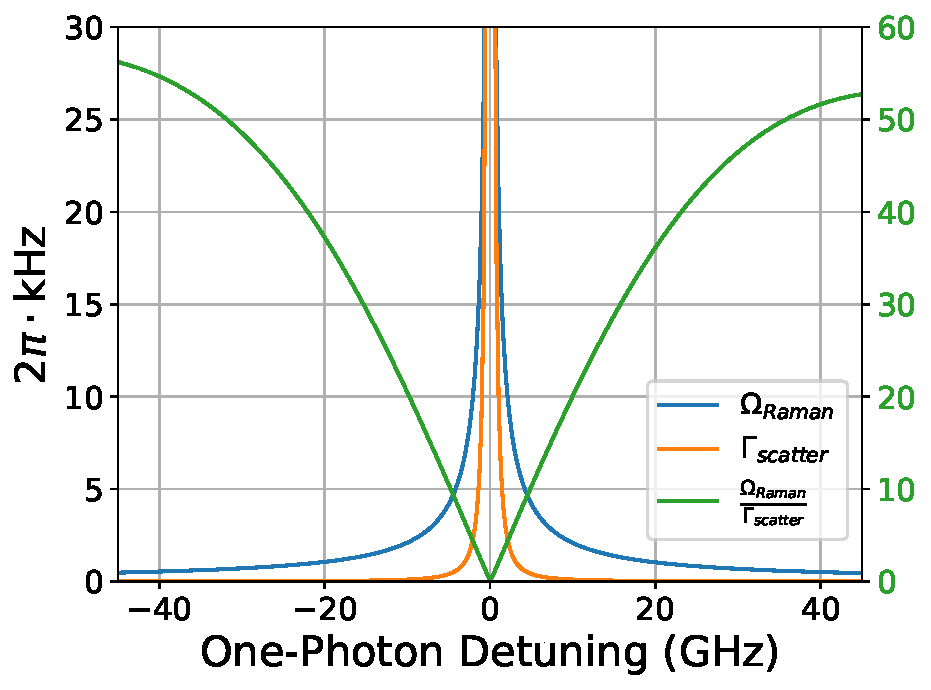
\includegraphics[width=5.4cm]{imgs/raman_v0.pdf}
        };
        \draw[->, blue, line width=2] (ThresholdPlot) -- (ThresholdHighlight);
        \draw[->, blue, line width=2] (DeepPlot) -- (DeepHighlight);
      }
    \end{tikzpicture}
  \end{center}
\end{frame}


%% Experiment
% Based on the comparison, we selected the ground vibrational state
% in the excited state (v=0), which we have already observed previously.
% And for the ground molecular state, the binding energy was predicted as
% ~771 MHz by Jeremy Hutson from Durham, based on our interaction shift
% and FB measurement. (Phys. Rev. Research 2, 023108 (2020))

% Thanks to the prediction, it didn't take too long for us to find the resonance.
% which was ~1MHz from the prediction.

% More importantly and different from all previous spectrum though,
% the 8.4 kHz FWHM is very closed to the Fourier limited linewidth
% for the 0.1 ms pulse time we use, suggesting that we are very closed to the coherent regime.

% So next we switched to scanning the time on resonance.
% And long and behold we see a revival in our signal, which is the evidence that
% we can drive the atoms to molecule and then back coherently.
% This is the first time coherent optical transfer has been done
% without using a narrow optical transition and we believe it can be applied to
% many other systems.

% The contrast is obviously not 100%, however, this actually correspond to
% 50% of initial ground state atom being transfered into molecular state.
% We believe the major contribitor to this contrast is the molecular lifetime
% which we measured here to be much shorter than what we expect.

% From the design of our transfer scheme, all molecules we made are in a single spin state
% with 50% or even more of them in the ground motional state.

\begin{frame}[t]{Experiment}
  \begin{center}
    \vspace{-0.9cm}
    \begin{tikzpicture}
      \visible<-4>{
        \begin{scope}[shift={(-5.5, -3.5)}, scale=0.8]
          \draw[->,line width=1.2] (0, 0) -- (0, 8);
          \node[above,rotate=90] at (0, 4) {Energy};
          \draw[->,line width=1.2] (0, 0) -- (5.4, 0);
          \node[below] at (2.7, -0.1) {Internuclear distance};

          \draw[line width=1.1,cyan!85!blue]
          plot[samples=200,domain=0.96:7,variable=\x]
          ({(\x + 0.25) * 0.7}, {(6.8*\x^(-3.4)-6.5*\x^(-1.7)) * 1.3 + 2.5});

          \draw[line width=1.1,red]
          plot[samples=200,domain=1:7.5,variable=\x]
          ({(\x - 0.75) * 0.7}, {(9.2*\x^(-2.5)-9.0*\x^(-1.3)) * 1.3 + 7.5});
          \node[above right,red] at (0.55 * 0.7, 7.2) {$c^3\Sigma^+$};

          \draw[red] ({(1.4 - 0.75) * 0.7}, -1.8 * 1.3 + 7.5) --
          ({(2.5 - 0.75) * 0.7}, -1.8 * 1.3 + 7.5) node[right=0.2] {\scriptsize $v=0$};
          \draw[black!40,dashed,line width=1] ({(1.2 - 0.75) * 0.7}, -2 * 1.3 + 7.5) --
          ({(3 - 0.75) * 0.7}, -2 * 1.3 + 7.5);

          \draw[cyan!85!blue] ({(1.0269 + 0.25) * 0.7}, 2.5) -- (7.25 * 0.7, 2.5);
          \mytweezer.drawNaAtom(6.55 * 0.7, 2.6, 0.12)
          \mytweezer.drawCsAtom(7.05 * 0.7, 2.6, 0.10)

          \draw[cyan!85!blue] ({(1.0793 + 0.25) * 0.7}, -0.28 * 1.3 + 2.5) -- ({(6 + 0.25) * 0.7}, -0.28 * 1.3 + 2.5);
          \mytweezer.drawNaAtom(4.08 * 0.7, -0.19  * 1.3 + 2.5, 0.12)
          \mytweezer.drawCsAtom(4.25 * 0.7, -0.19  * 1.3 + 2.5, 0.10)

          \draw[->,blue!50!orange,line width=0.8] (6.8 * 0.7, 2.7)
          -- node[right] {$\Omega_{up}$} ({(2.8 - 0.75) * 0.7}, -2 * 1.3 + 7.5);
          \draw[->,green!80!black,line width=0.8] ({(2.75 - 0.75) * 0.7}, -2 * 1.3 + 7.5)
          -- node[left] {$\Omega_{down}$} (4.165 * 0.7, -0.12 * 1.3 + 2.5);

          \draw[->,cyan!55!blue, line width=1] (5.1 * 0.7, 3) -- (5.1 * 0.7, 2.5);
          \draw[<-,cyan!55!blue, line width=1] (5.1 * 0.7, -0.28 * 1.3 + 2.5)
          -- (5.1 * 0.7, -0.28 * 1.3 + 2)
          node[below, align=center] {\scriptsize $\approx771\mathrm{MHz}$\\
            \scriptsize by Jeremy Hutson.};
        \end{scope}
      }
      \visible<2> {
        \node[below] at (2.6, 4) {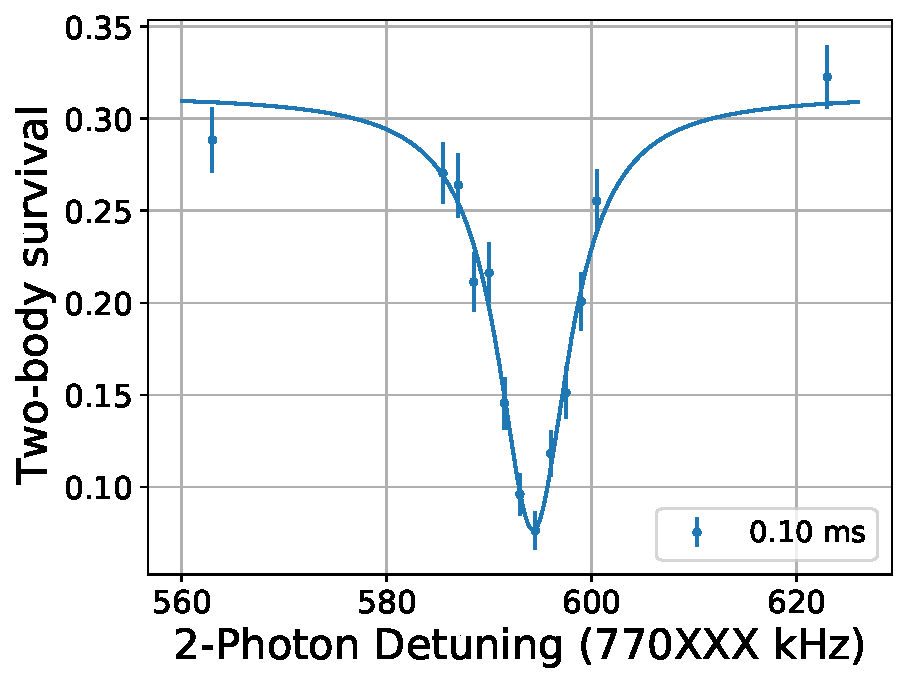
\includegraphics[width=5.5cm]{../../experiments/nacs_202003/imgs/fit_20200326_005204_raman_3322_2_damop_f.pdf}};
      }
      \visible<3-> {
        \node[below] at (2.6, 4) {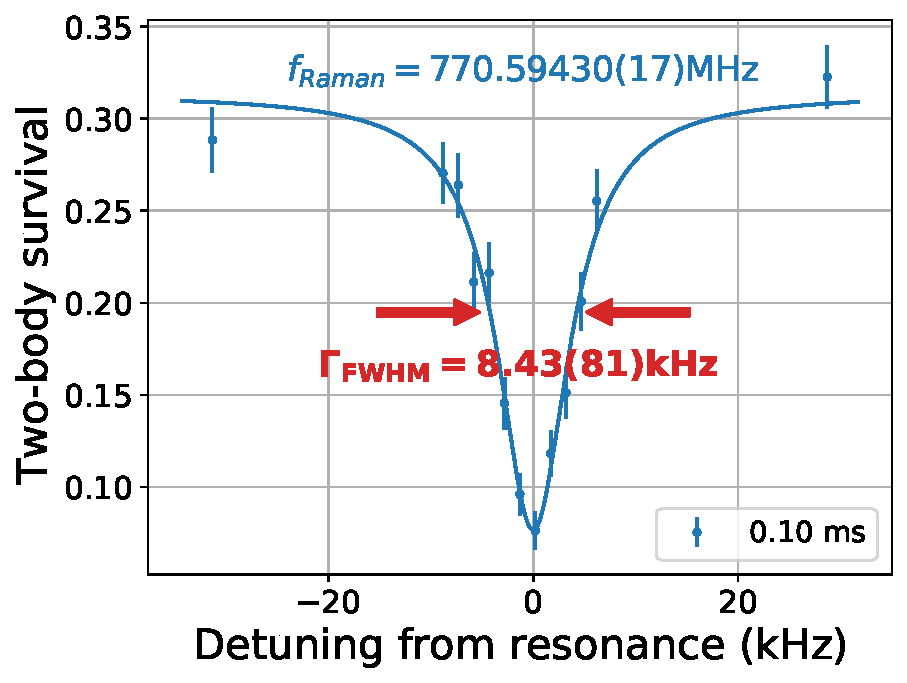
\includegraphics[width=5.5cm]{../../experiments/nacs_202003/imgs/fit_20200326_005204_raman_3322_2_damop_f_text.pdf}};
      }
      \visible<4-5> {
        \node[below] at (2.6, -0.5) {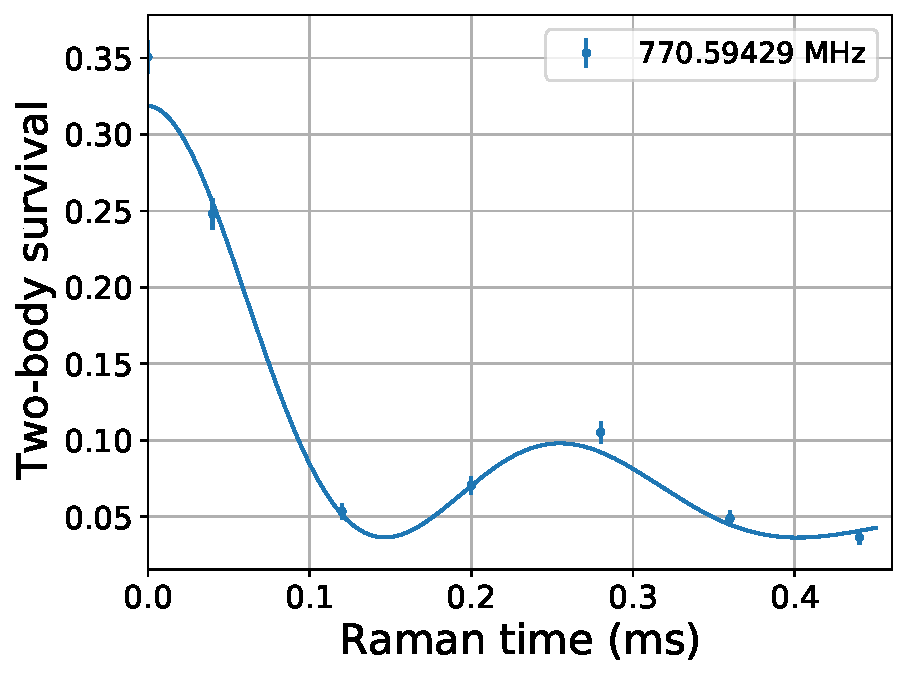
\includegraphics[width=5.5cm]{../../experiments/nacs_202003/imgs/fit_20200326_005204_raman_3322_2_damop_t.pdf}};
      }
      \visible<6-> {
        \node[below] at (2.6, -0.5) {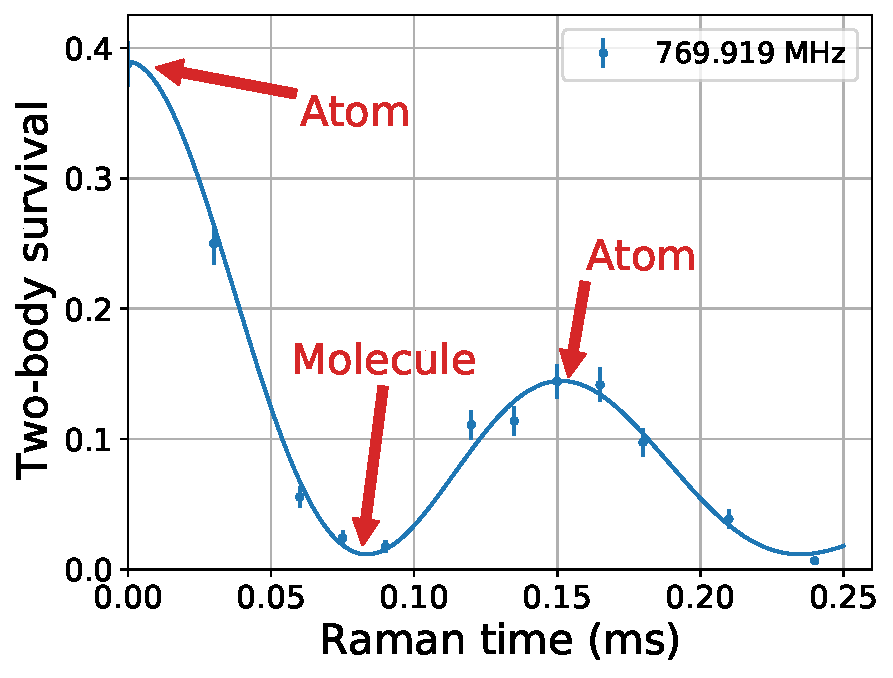
\includegraphics[width=5.5cm]{../../experiments/nacs_202007/imgs/fit_20200703_201618_raman15_3322_2_postdoc_t.pdf}};
      }
      \visible<5-> {
        \node[below, text width=5.5cm, align=center] at (-3, 3.4)
        {
          \begin{itemize}
          \item Transferred \alt<-6>{$50\%$}{$65\%$} of ground state atom to molecule.
          \item<8-> Single molecule spin state
          \item<8-> $>50\%$ of molecule in motional ground state.
          \end{itemize}
        };
      }
      \visible<5-6> {
        \node[below] at (-3.2, 0.3) {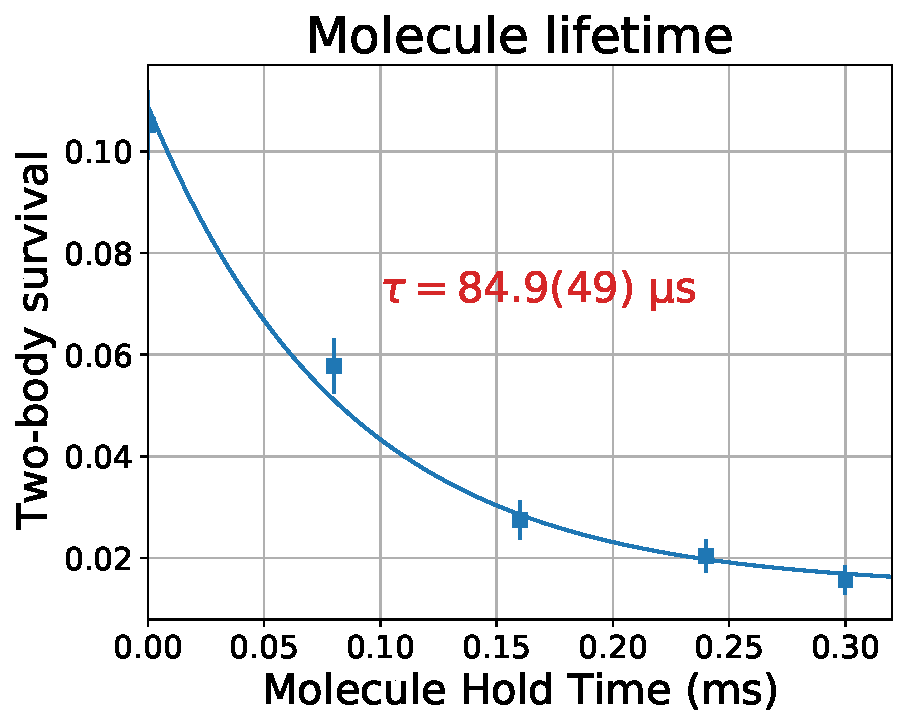
\includegraphics[width=5.3cm]{../../experiments/nacs_202003/imgs/fit_20200326_005204_raman_3322_2_damop_m_t.pdf}};
      }
      \visible<7-> {
        \node[below] at (-3.2, 0.3) {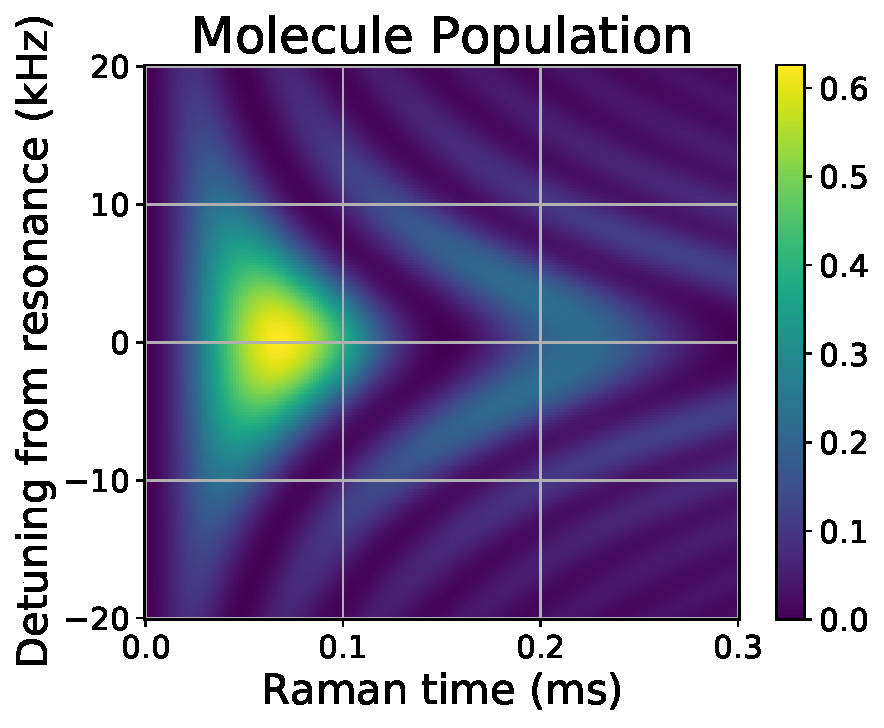
\includegraphics[width=5.3cm]{../../experiments/nacs_202007/imgs/fit_20200703_201618_raman15_3322_2_postdoc_2d_mol.pdf}};
      }
    \end{tikzpicture}
  \end{center}
\end{frame}

\section{Conclusion}
%% Conclusion
% * Experiment aiming to create flexible array of ultracold molecules for applications like ...
% * Atomic state preparation (internal and external, and how we overcome the challenge for Na)
% * Molecular state transfer (coherence, maintaining control, all optical)
% * Next step: transfer to ground state (could be from FB molecule).
\begin{frame}[t]{Conclusion and outlook}
  \vspace{-0.5cm}
  \begin{columns}
    \column{6cm}
    \begin{itemize}
    \item Full quantum control of atoms in optical tweezers
    \item Coherent all-optical creation of single molecucle
    \item<2-> Improve molecule lifetime and signal contrast
      % TODO: scaling, interaction/entanglement
    \item<3-> Feshbach molecule\\
      {\small $\left(\tau=4.7(7)\ \mathrm{ms}\right)$}
    \end{itemize}
    \column{5.8cm}
    \visible<4->{
      \begin{tikzpicture}
        %% PI
        \node[align=center] at (0, -0.8) {Experiment};
        \node[below,align=center, execute at begin node=\setlength{\baselineskip}{7pt}] at (2, 0)
        {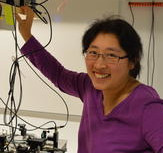
\includegraphics[height=1.5cm]{kangkuen}\\\scriptsize Kang-Kuen Ni};

        %% Current member
        \node[below,align=center, execute at begin node=\setlength{\baselineskip}{7pt}] at (-1.5, -2.2)
        {\includegraphics[height=1.5cm]{kenneth}\\\scriptsize Kenneth\\\scriptsize Wang};
        \node[below,align=center, execute at begin node=\setlength{\baselineskip}{7pt}] at (0, -2.2)
        {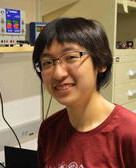
\includegraphics[height=1.5cm]{jessie}\\\scriptsize Jessie\\\scriptsize Zhang};
        \node[below,align=center, execute at begin node=\setlength{\baselineskip}{7pt}] at (1.5, -2.2)
        {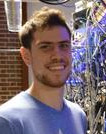
\includegraphics[height=1.5cm]{lewis}\\\scriptsize Lewis\\\scriptsize Picard};
        \node[below,align=center, execute at begin node=\setlength{\baselineskip}{7pt}] at (3.0, -2.2)
        {\includegraphics[height=1.5cm]{will}\\\scriptsize William\\\scriptsize Cairncross};

        %% Former member
        \node[below,align=center, execute at begin node=\setlength{\baselineskip}{7pt}] at (-1.5 + 0.375, -4.4)
        {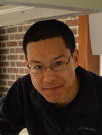
\includegraphics[height=1.5cm]{lee}\\\scriptsize Lee Liu\\\tiny Postdoc @JILA};
        \node[below,align=center, execute at begin node=\setlength{\baselineskip}{7pt}] at (0.75, -4.4)
        {\includegraphics[height=1.5cm]{jon}\\\scriptsize Jonathan Hood\\\tiny Assnt Prof @Purdue};
        \node[below,align=center, execute at begin node=\setlength{\baselineskip}{7pt}] at (3 - 0.375, -4.4)
        {\includegraphics[height=1.5cm]{nick}\\\scriptsize Nick Hutzler\\\tiny Assnt Prof @Caltech};

        %% Theory
        \node[below,align=center] at (0, -7.1) {Theory};
        \node[below,align=center, execute at begin node=\setlength{\baselineskip}{7pt}] at (1.7, -6.6)
        {\includegraphics[height=1.5cm]{jeremy}\\\scriptsize Jeremy Hutson};
      \end{tikzpicture}
    }
  \end{columns}
\end{frame}

\begin{frame}{}
\end{frame}

\begin{frame}{}
\end{frame}

%% Backup slides

\end{document}
